\documentclass[aspectratio=169]{beamer}

\usepackage{fontspec}
\usepackage{microtype}
\usepackage{fontawesome}
\usepackage{emoji}

\hypersetup{
    colorlinks,
    linkcolor=red,
    pdftitle={Dark Corner of STL},
    pdfpagemode=FullScreen,
    }

\setmonofont{JetBrainsMono}[
    Path=./static/fonts/jetbrains/,
    Scale=0.85,
    Extension = .ttf,
    UprightFont=*-Regular,
    BoldFont=*-Bold,
    ItalicFont=*-Italic,
    BoldItalicFont=*-BoldItalic
    ]
    
\setsansfont{Asap}[
    Path=./static/fonts/asap/,
    Scale=0.9,
    Extension = .ttf,
    UprightFont=*-Regular,
    BoldFont=*-Bold,
    ItalicFont=*-Italic,
    BoldItalicFont=*-BoldItalic
    ]
    
\usepackage[newfloat=true]{minted}
\usemintedstyle{xcode}
\beamertemplatenavigationsymbolsempty

\setbeamertemplate{footline}{\begin{center}\quad\insertframenumber\strut\quad\end{center}}
\setbeamerfont{footline}{size=\large}

%\setbeameroption{hide notes} % Only slides
%\setbeameroption{show only notes} % Only notes
%\setbeameroption{show notes on second screen=left}

\title{Living comfortably at HEAD with Bazel}
\author{Šimon Tóth}

\begin{document}

\begin{frame}{}
    \titlepage
\end{frame}

\begin{frame}{}
\begin{center}
        \Large\href{https://github.com/HappyCerberus/meetingcpp22-bazel}{https://github.com/HappyCerberus/meetingcpp22-bazel}\\
        
\includegraphics[width=.4\textwidth]{static/qrcode.png}
\end{center}
\end{frame}

\begin{frame}{}
    \begin{columns}
        \begin{column}{0.35\textwidth}
            
\includegraphics[height=0.8\textheight]{static/book_cover.png}
        \end{column}
        \begin{column}{0.6\textwidth}
            \begin{itemize}
                \item Free on GitHub:\\
                    \href{https://github.com/HappyCerberus/book-cpp-algorithms}{HappyCerberus/book-cpp-algorithms}
                \item Donate to EFF on LeanPub:\\
                    \href{https://leanpub.com/cpp-algorithms-guide}{leanpub.com/cpp-algorithms-guide}
            \end{itemize}
        \end{column}
    \end{columns}
\end{frame}

\begin{frame}{}
\begin{columns}
    \begin{column}{0.35\textwidth}
    \begin{itemize}
        \item \href{https://twitter.com/SimonToth83}{twitter.com/SimonToth83}
        \item \href{https://www.linkedin.com/in/simontoth}{linkedin.com/in/simontoth}
    \end{itemize}
    \end{column}
    \begin{column}{0.60\textwidth}
        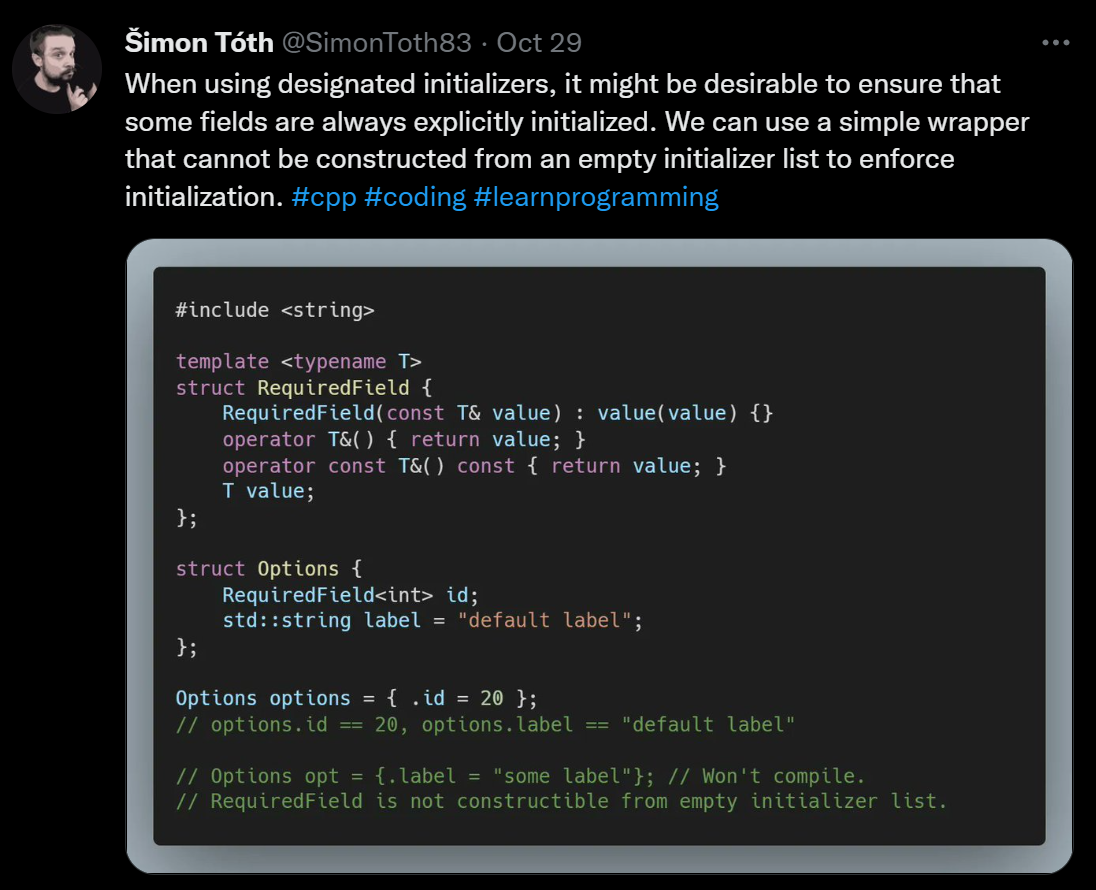
\includegraphics[width=\textwidth]{static/tweet.png}
    \end{column}
\end{columns}
\end{frame}

\begin{frame}{}
\begin{center}
    \begin{Huge}
        Monorepo vs Polyrepo
    \end{Huge}
\end{center}
\end{frame}

\begin{frame}{}
\Huge
\begin{center}
\begin{description}
    \item[mono-] one, single \pause
    \item[poly-] many
\end{description}
\end{center}
\end{frame}

\begin{frame}{}
\Huge
\begin{center}
\begin{description}
    \item[@HEAD] built from current sources \pause
    \item[binary] versioned binaries
\end{description}
\end{center}
\end{frame}

\begin{frame}{Comparison}
\begin{columns}
    \begin{column}{0.5\textwidth}
    @HEAD monorepo
    \begin{itemize}
        \item<2-> \emoji{face-with-head-bandage} scalability 
        \item<3-> \emoji{smirking-face} global operations are possible
        \item<4-> \emoji{grimacing-face} private dependencies are non-trivial
        \item<5-> \emoji{face-with-raised-eyebrow} shared dependencies need to be carefully managed
    \end{itemize}
    \end{column}
    \begin{column}{0.5\textwidth}
    binary polyrepo
    \begin{itemize}
        \item<2-> \emoji{anxious-face-with-sweat} ABI stability
        \item<3-> \emoji{exploding-head} global operations do not exist
        \item<4-> \emoji{smiling-face-with-smiling-eyes} private dependencies are trivial
        \item<5-> \emoji{frowning-face} shared dependencies need to be carefully managed
    \end{itemize}
    \end{column}
\end{columns}
\end{frame}

\begin{frame}{Comparison}
\begin{columns}
    \begin{column}{0.5\textwidth}
    @HEAD monorepo
    \begin{itemize}
        \item<2-> cooperative
        \item<3-> conforming
        \item<4-> biased towards users
    \end{itemize}
    \end{column}
    \begin{column}{0.5\textwidth}
    binary polyrepo
    \begin{itemize}
        \item<2-> competitive
        \item<3-> independent
        \item<4-> biased towards providers
    \end{itemize}
    \end{column}
\end{columns}
\end{frame}

\begin{frame}{}
\begin{center}
    \begin{Huge}
        Bazel
    \end{Huge}
\end{center}
\end{frame}

\begin{frame}{}
    \begin{center}
        \begin{Huge}Hello World Demo\end{Huge}
    \end{center}
\end{frame}

{
\usebackgroundtemplate{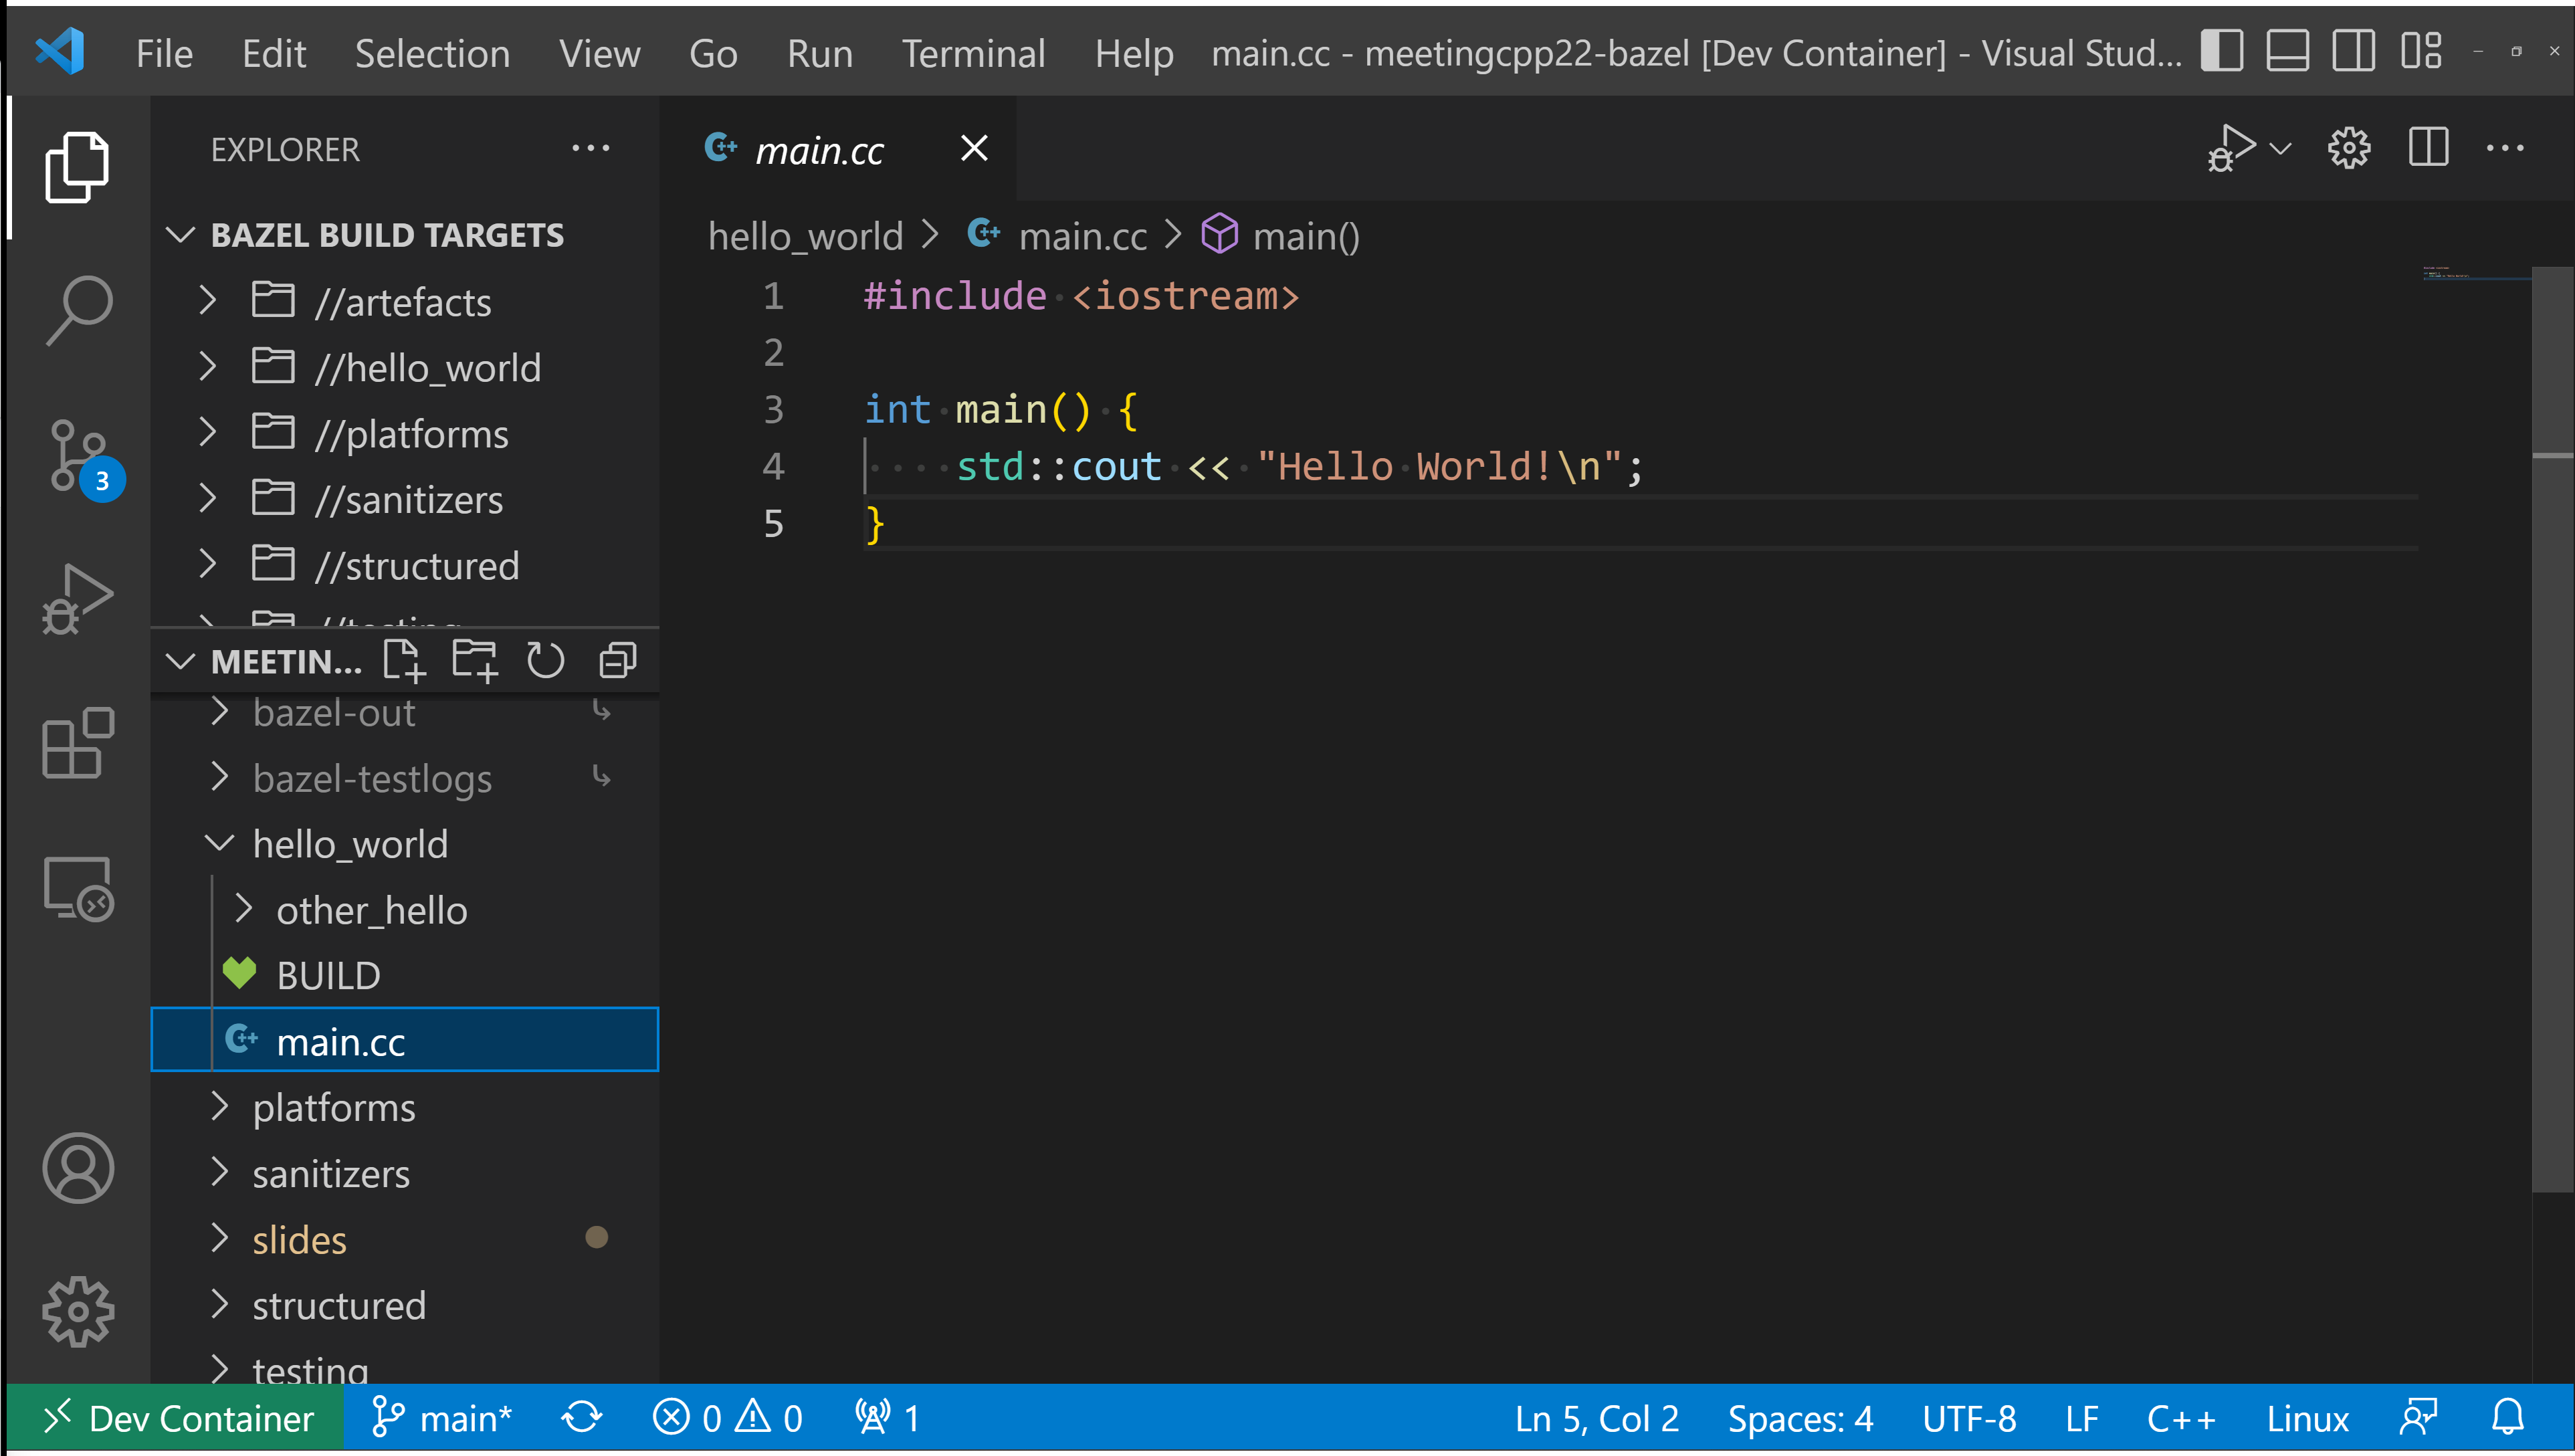
\includegraphics[width=\paperwidth]{slides/static_demos/00_01_hello_world.png}}
\begin{frame}[plain]
\end{frame}
}

{
\usebackgroundtemplate{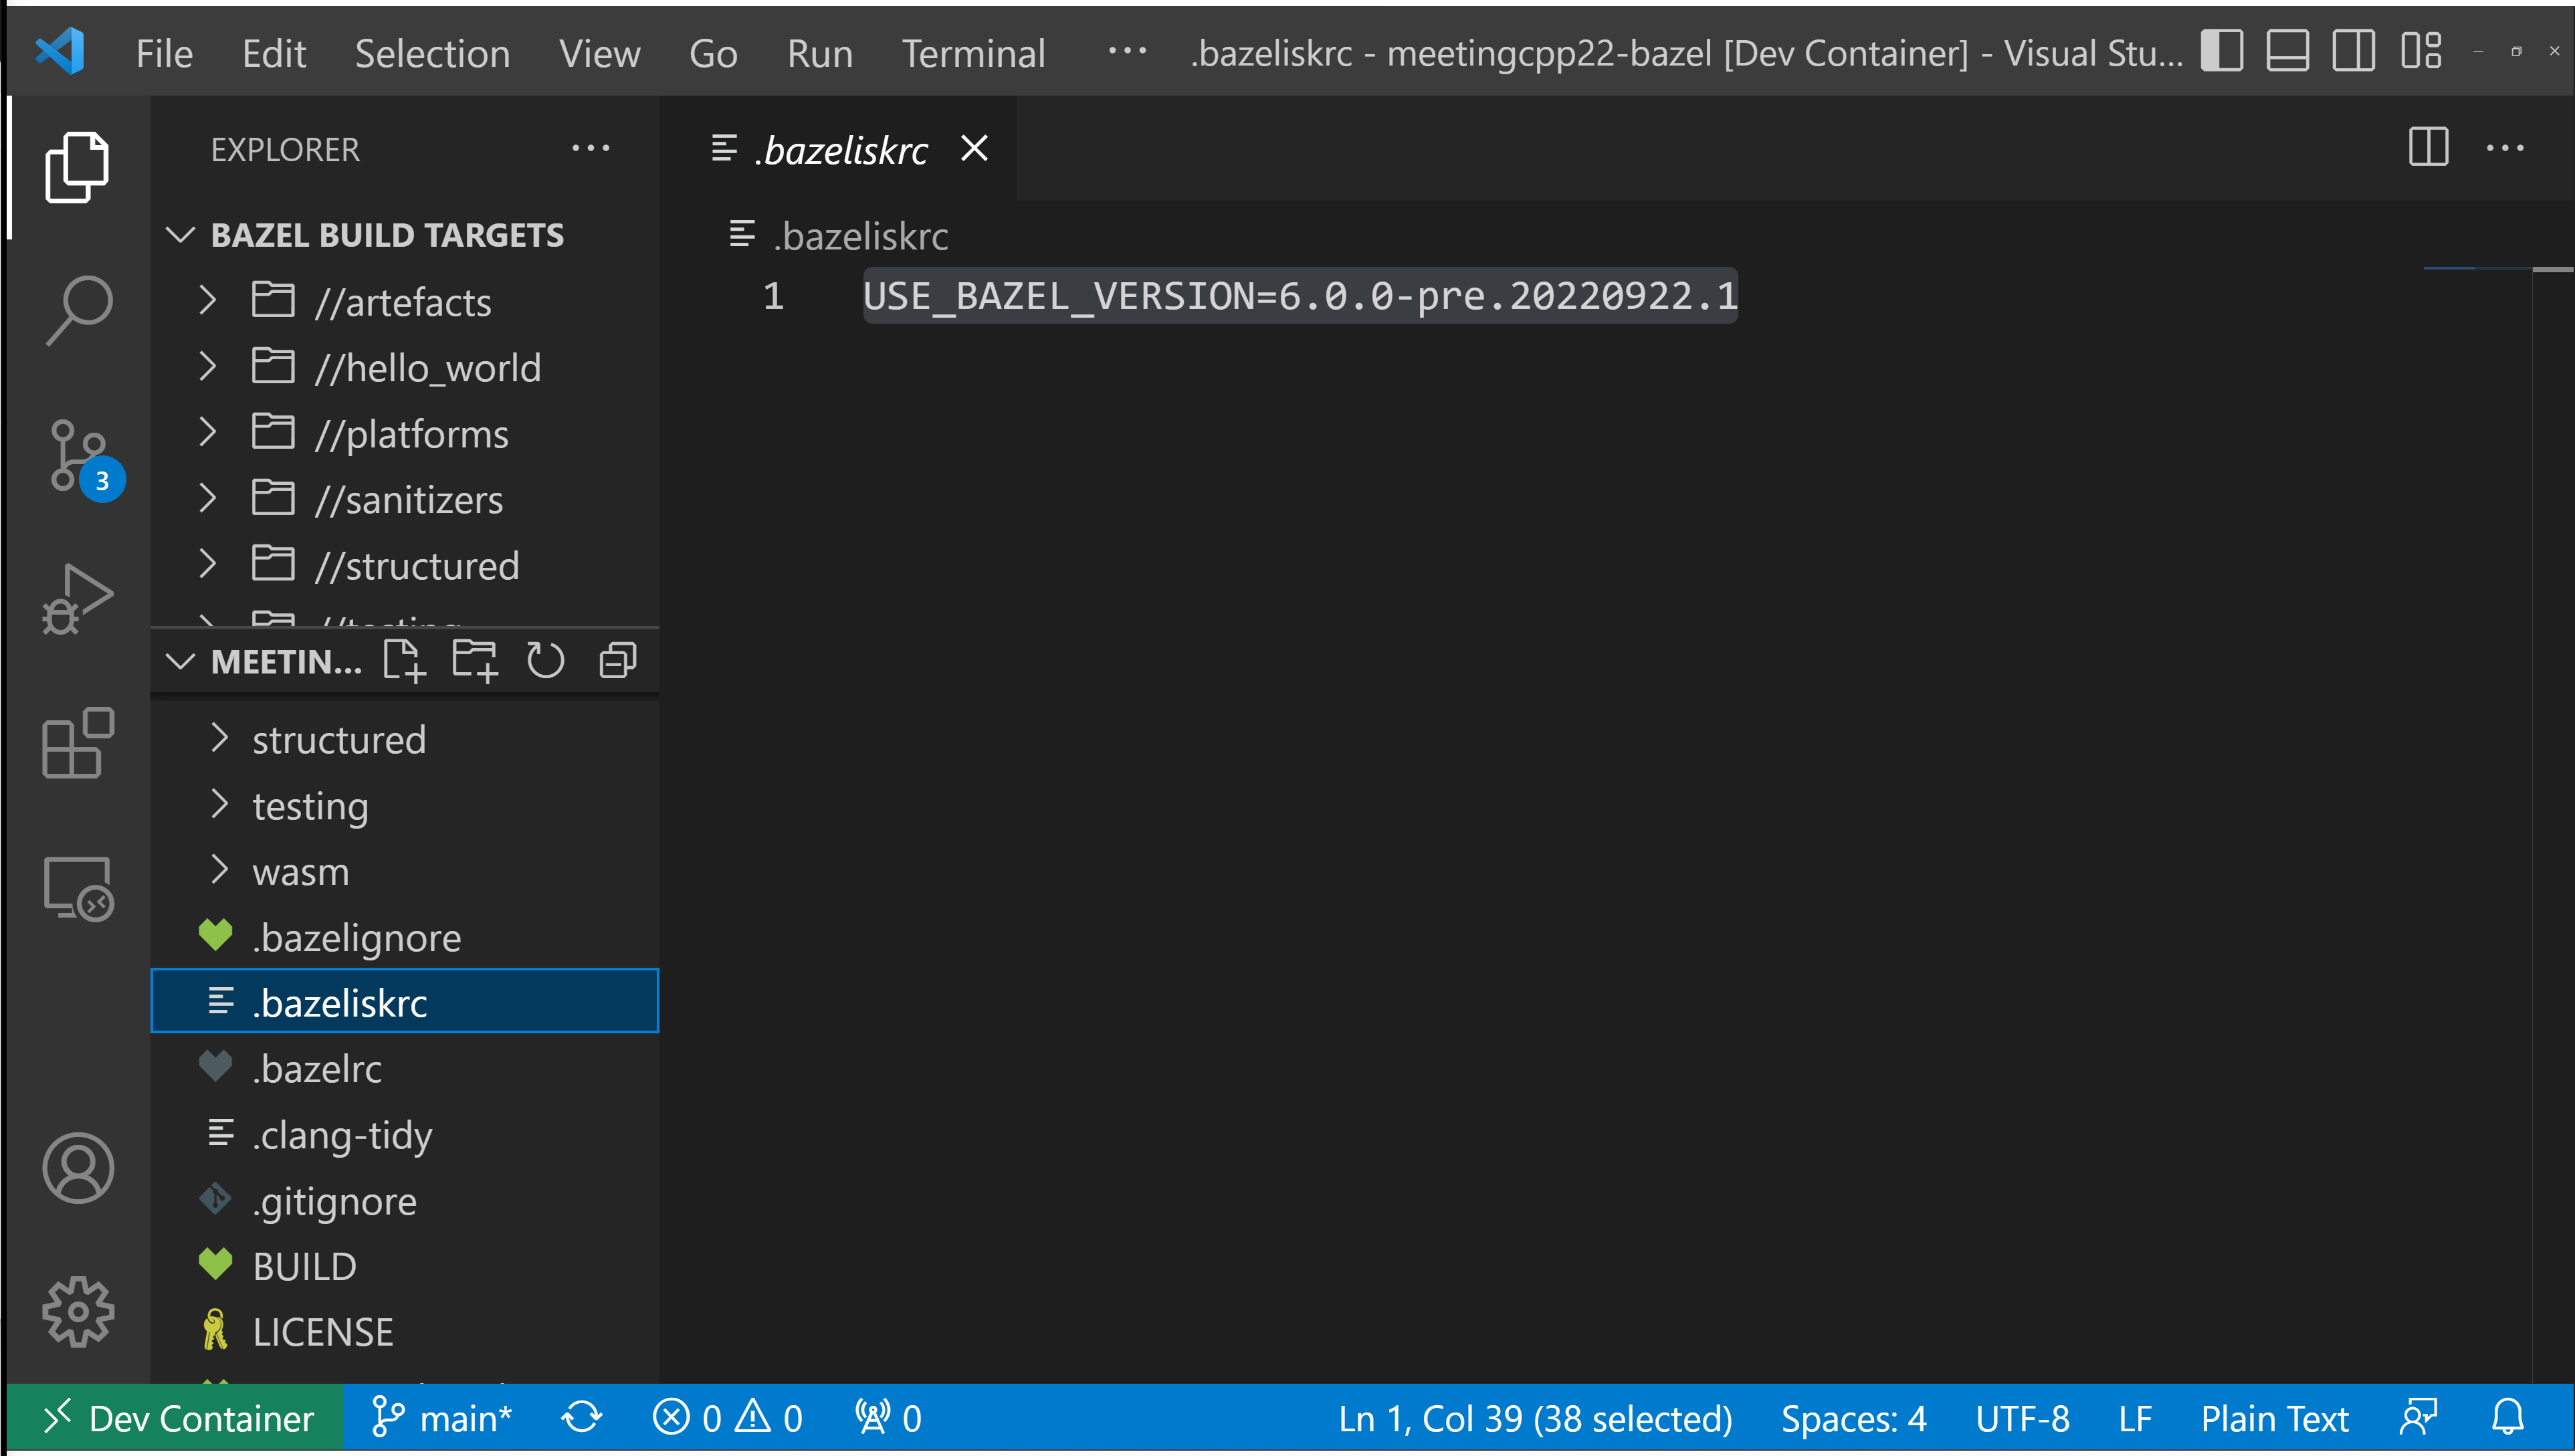
\includegraphics[width=\paperwidth]{slides/static_demos/00_02_bazeliskrc.png}}
\begin{frame}[plain]
\end{frame}
}

{
\usebackgroundtemplate{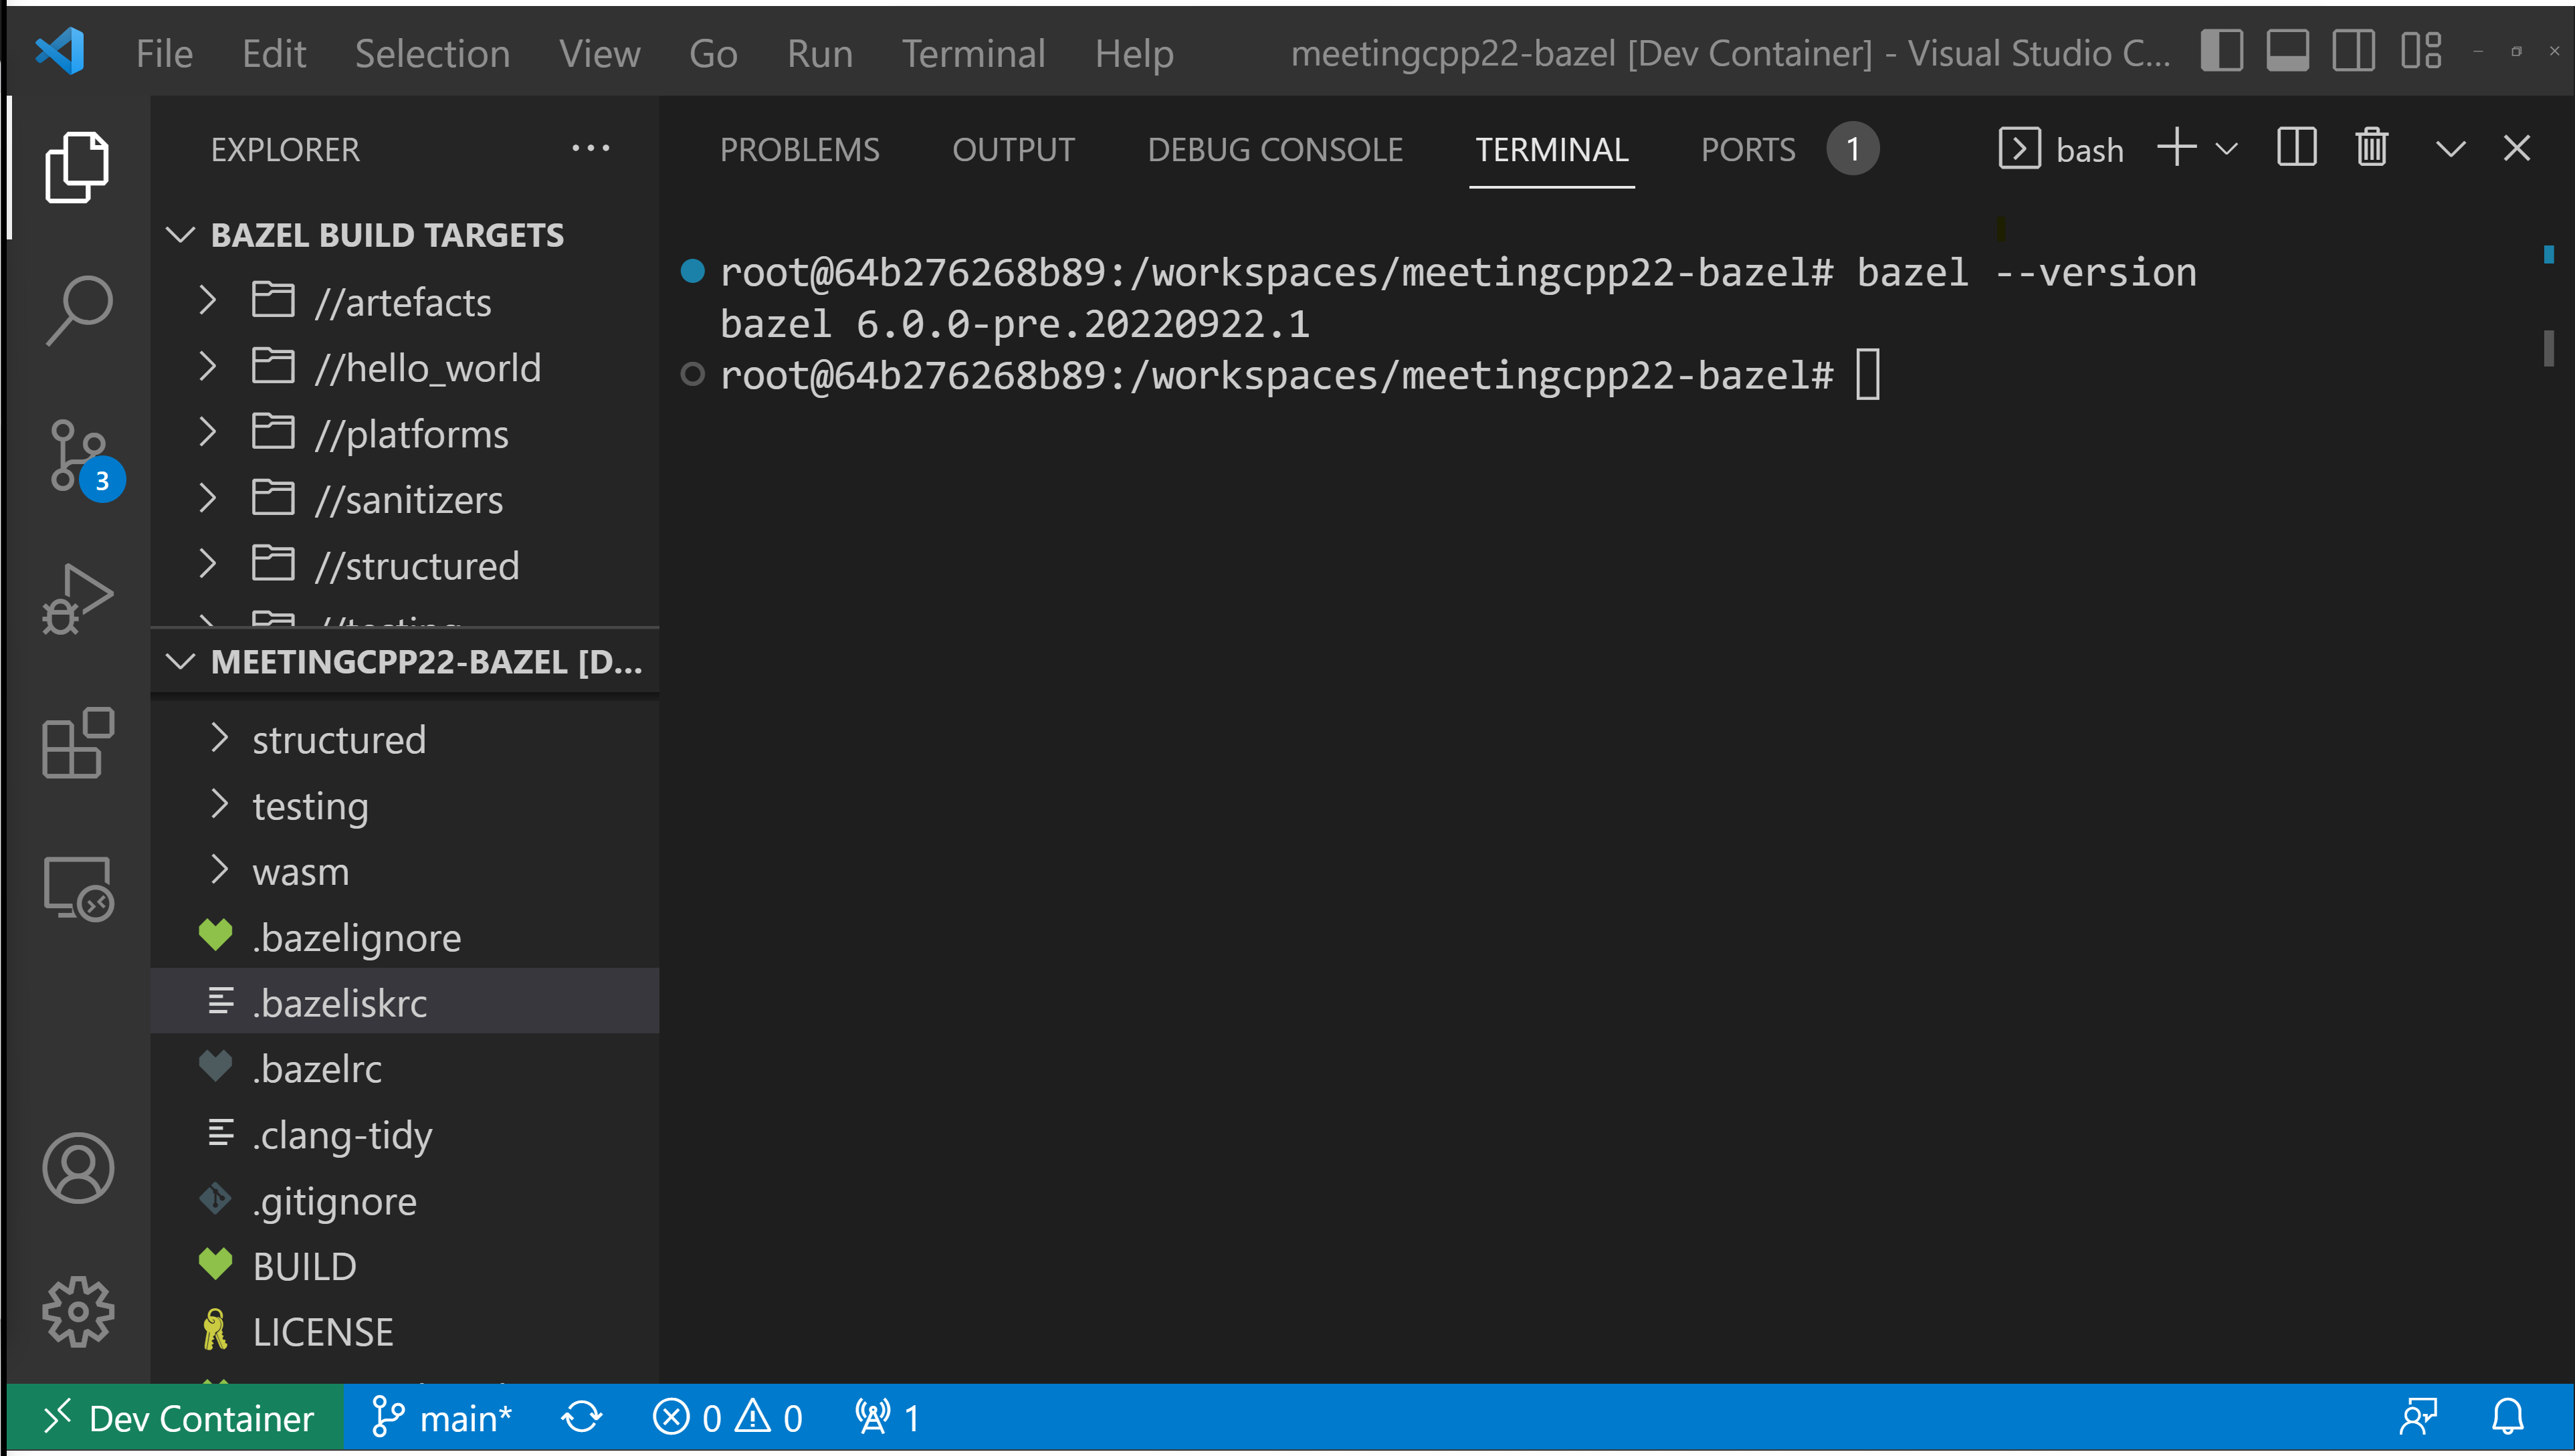
\includegraphics[width=\paperwidth]{slides/static_demos/00_03_bazel_version.png}}
\begin{frame}[plain]
\end{frame}
}

{
\usebackgroundtemplate{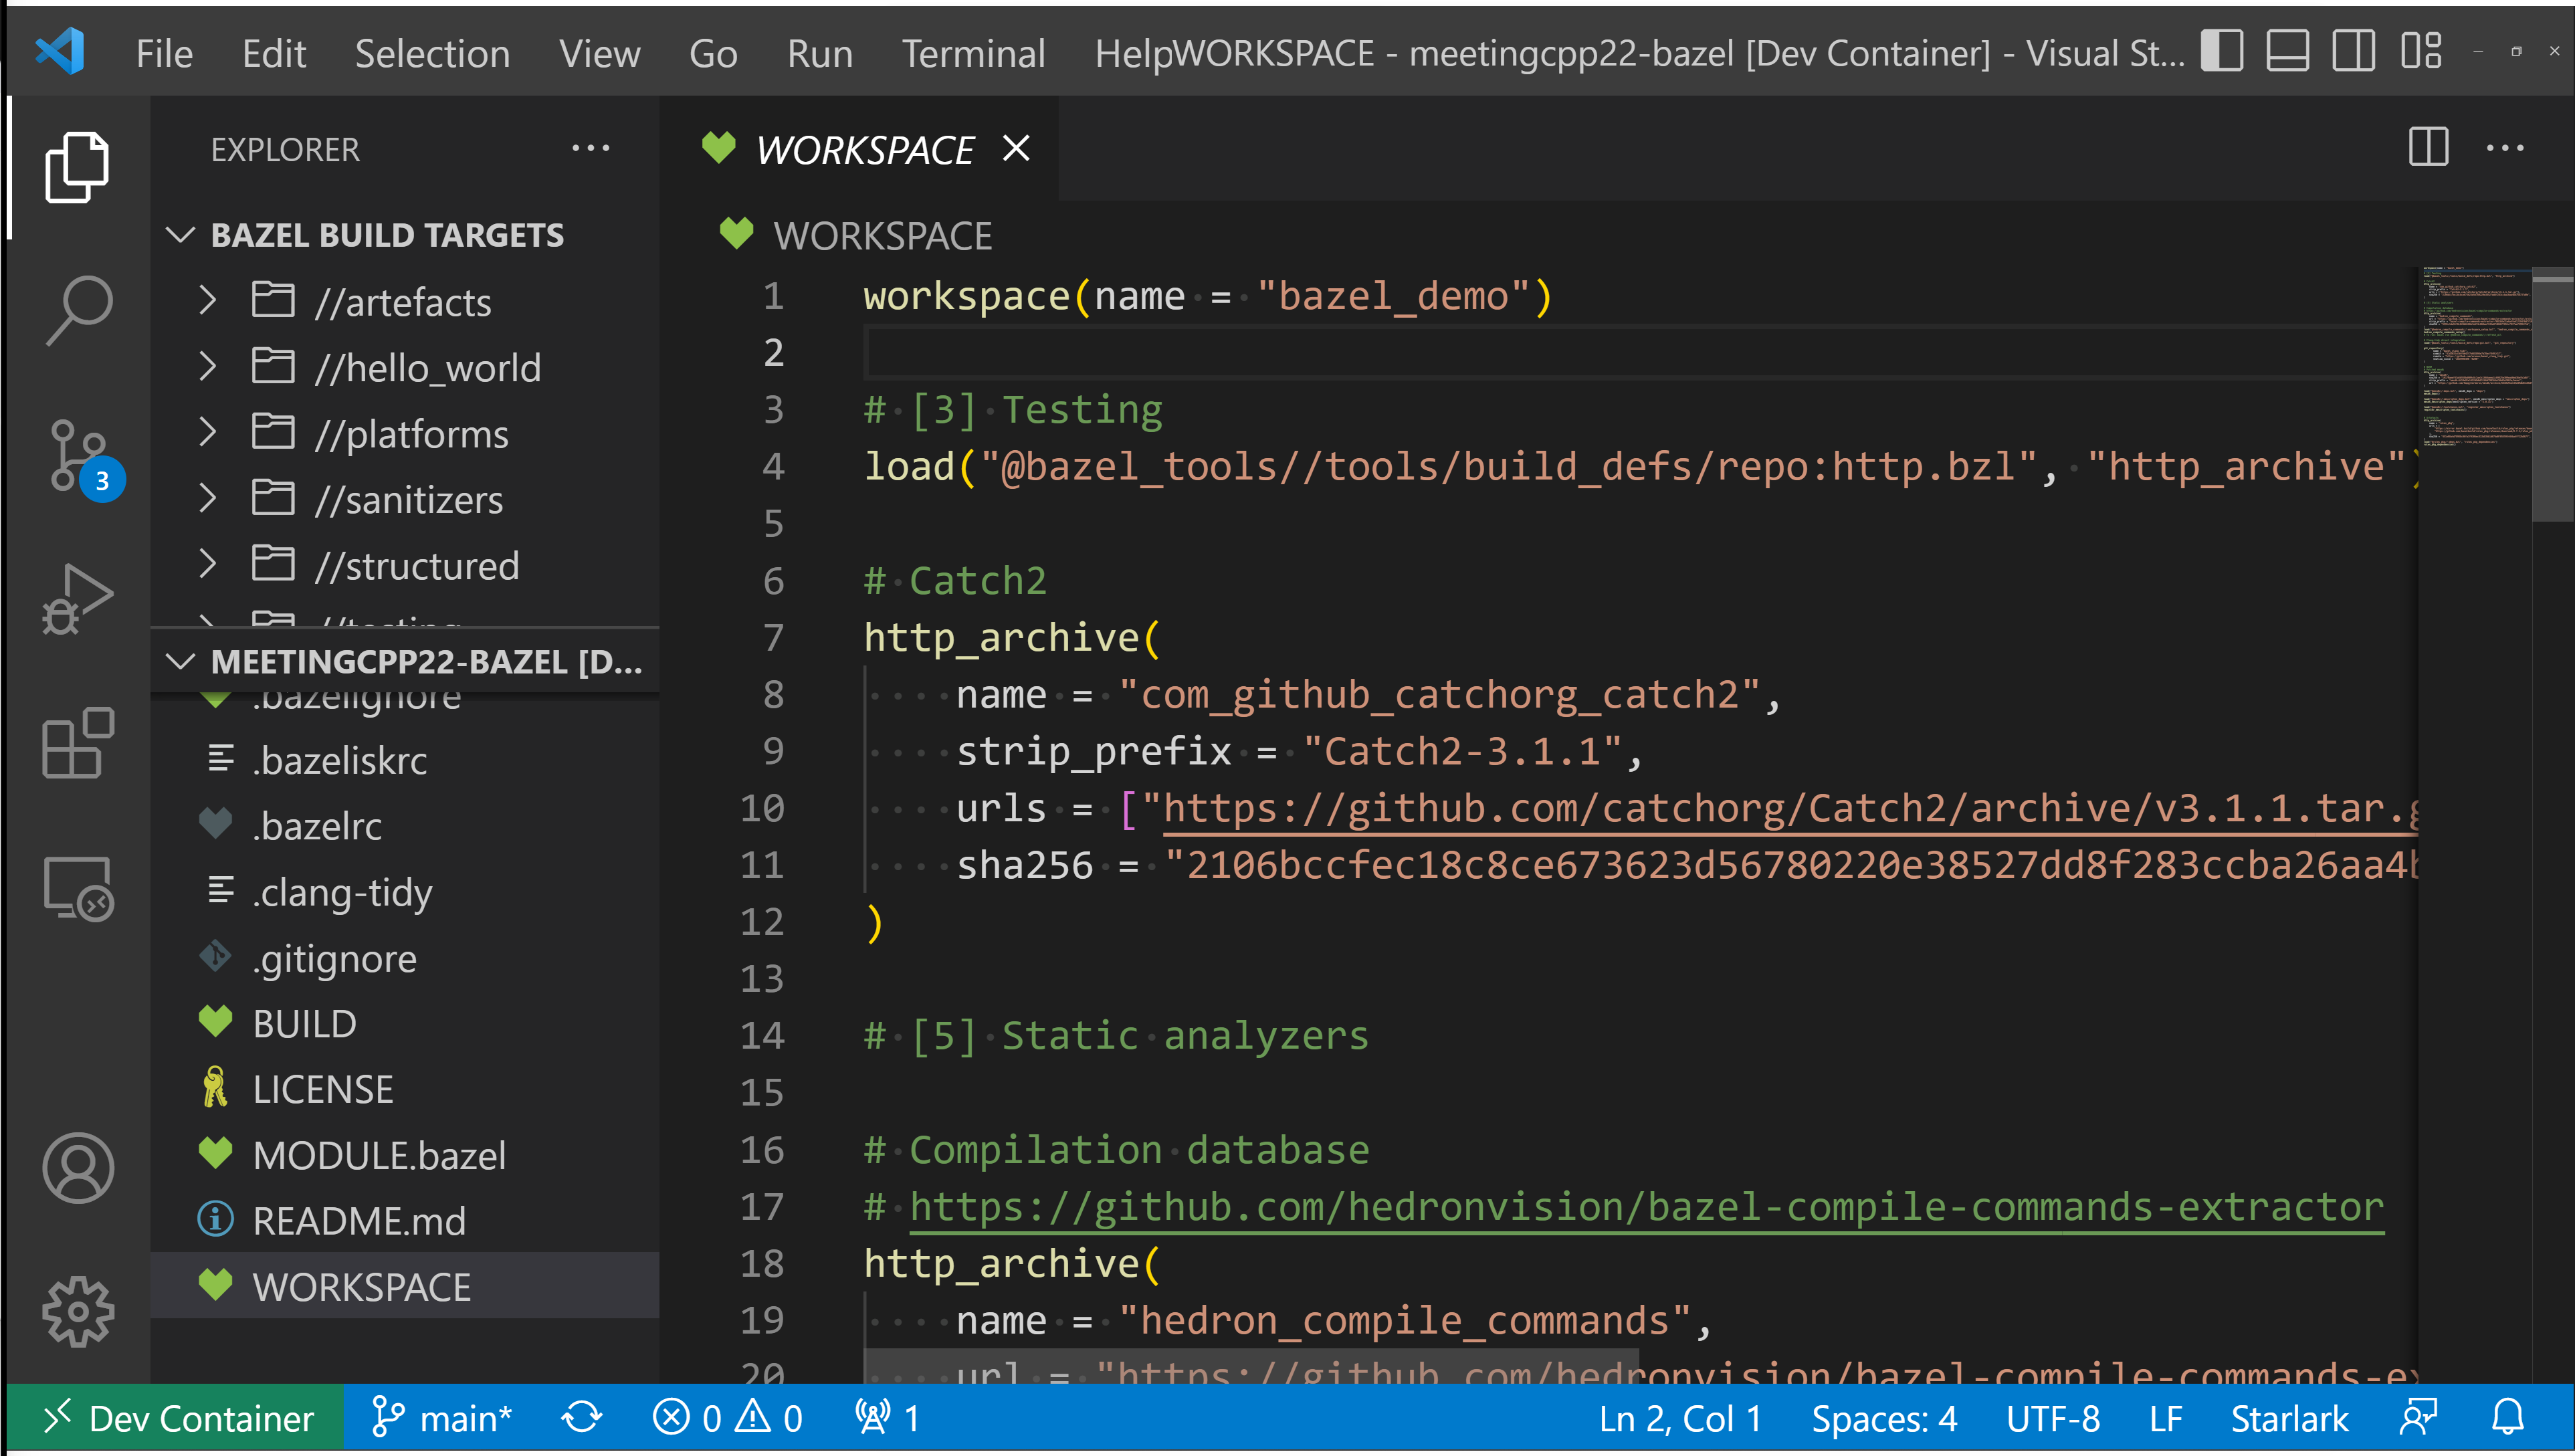
\includegraphics[width=\paperwidth]{slides/static_demos/00_04_WORKSPACE.png}}
\begin{frame}[plain]
\end{frame}
}

{
\usebackgroundtemplate{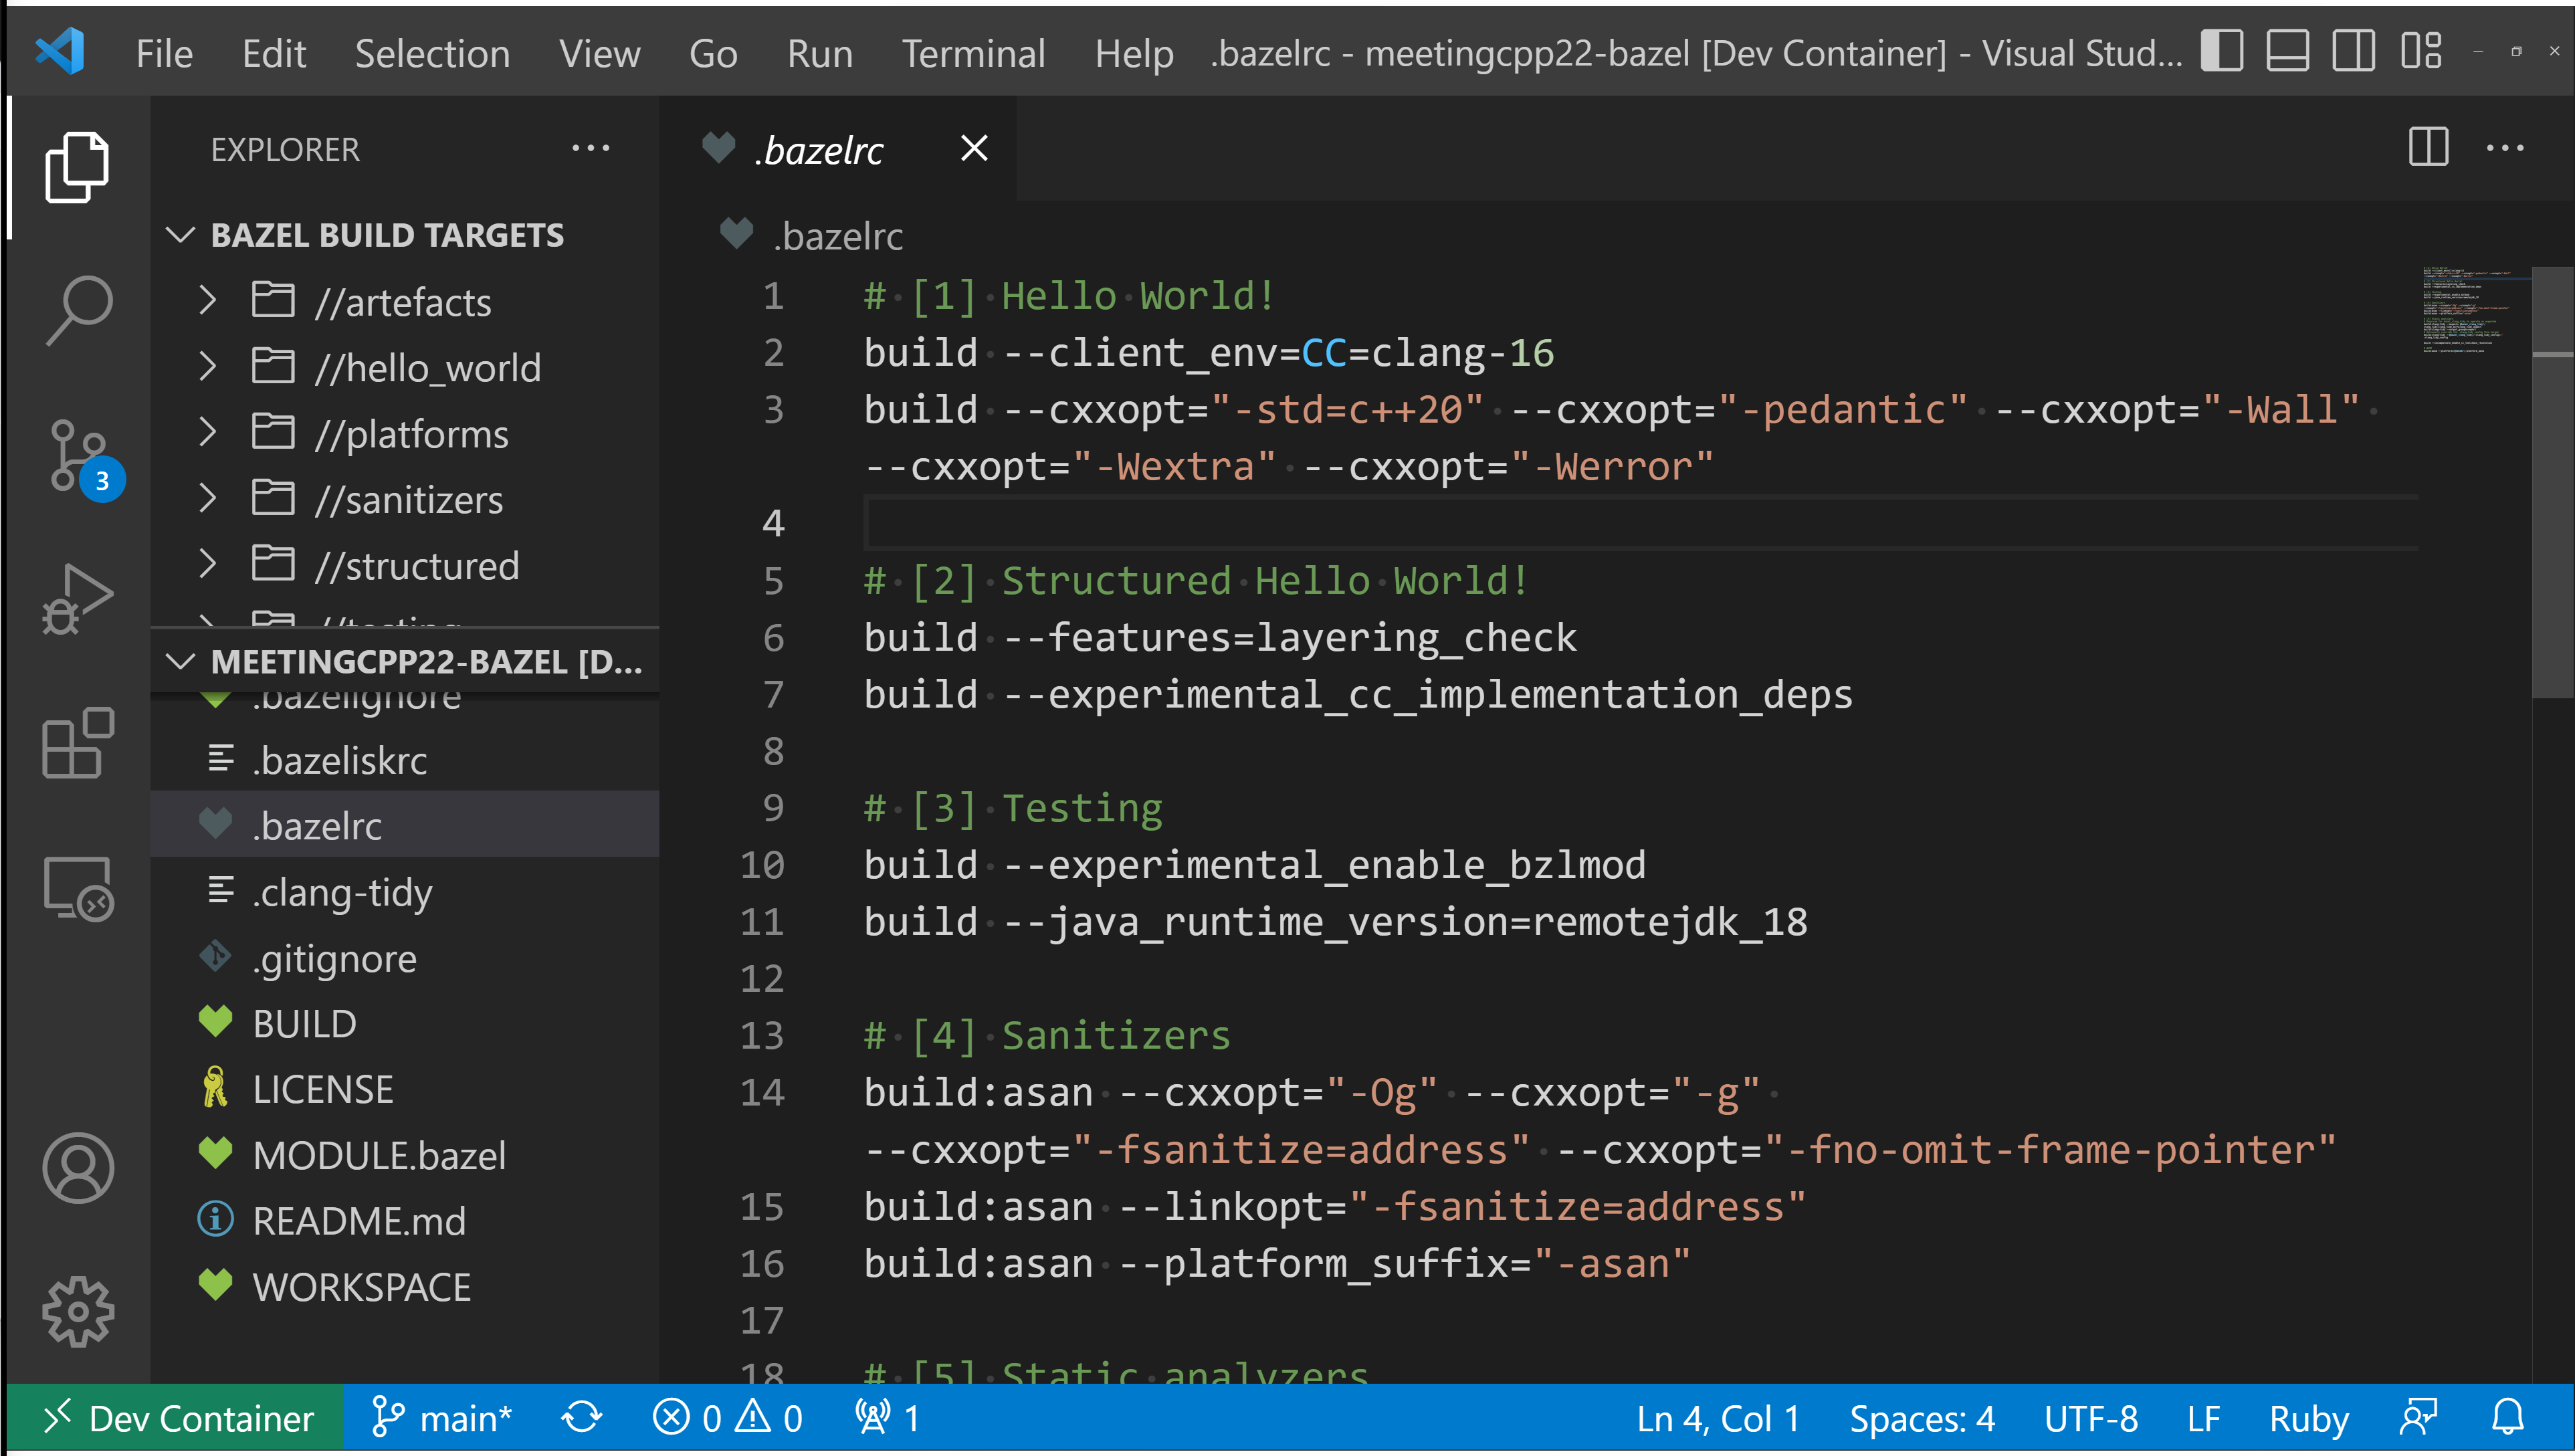
\includegraphics[width=\paperwidth]{slides/static_demos/00_05_bazelrc.png}}
\begin{frame}[plain]
\end{frame}
}

{
\usebackgroundtemplate{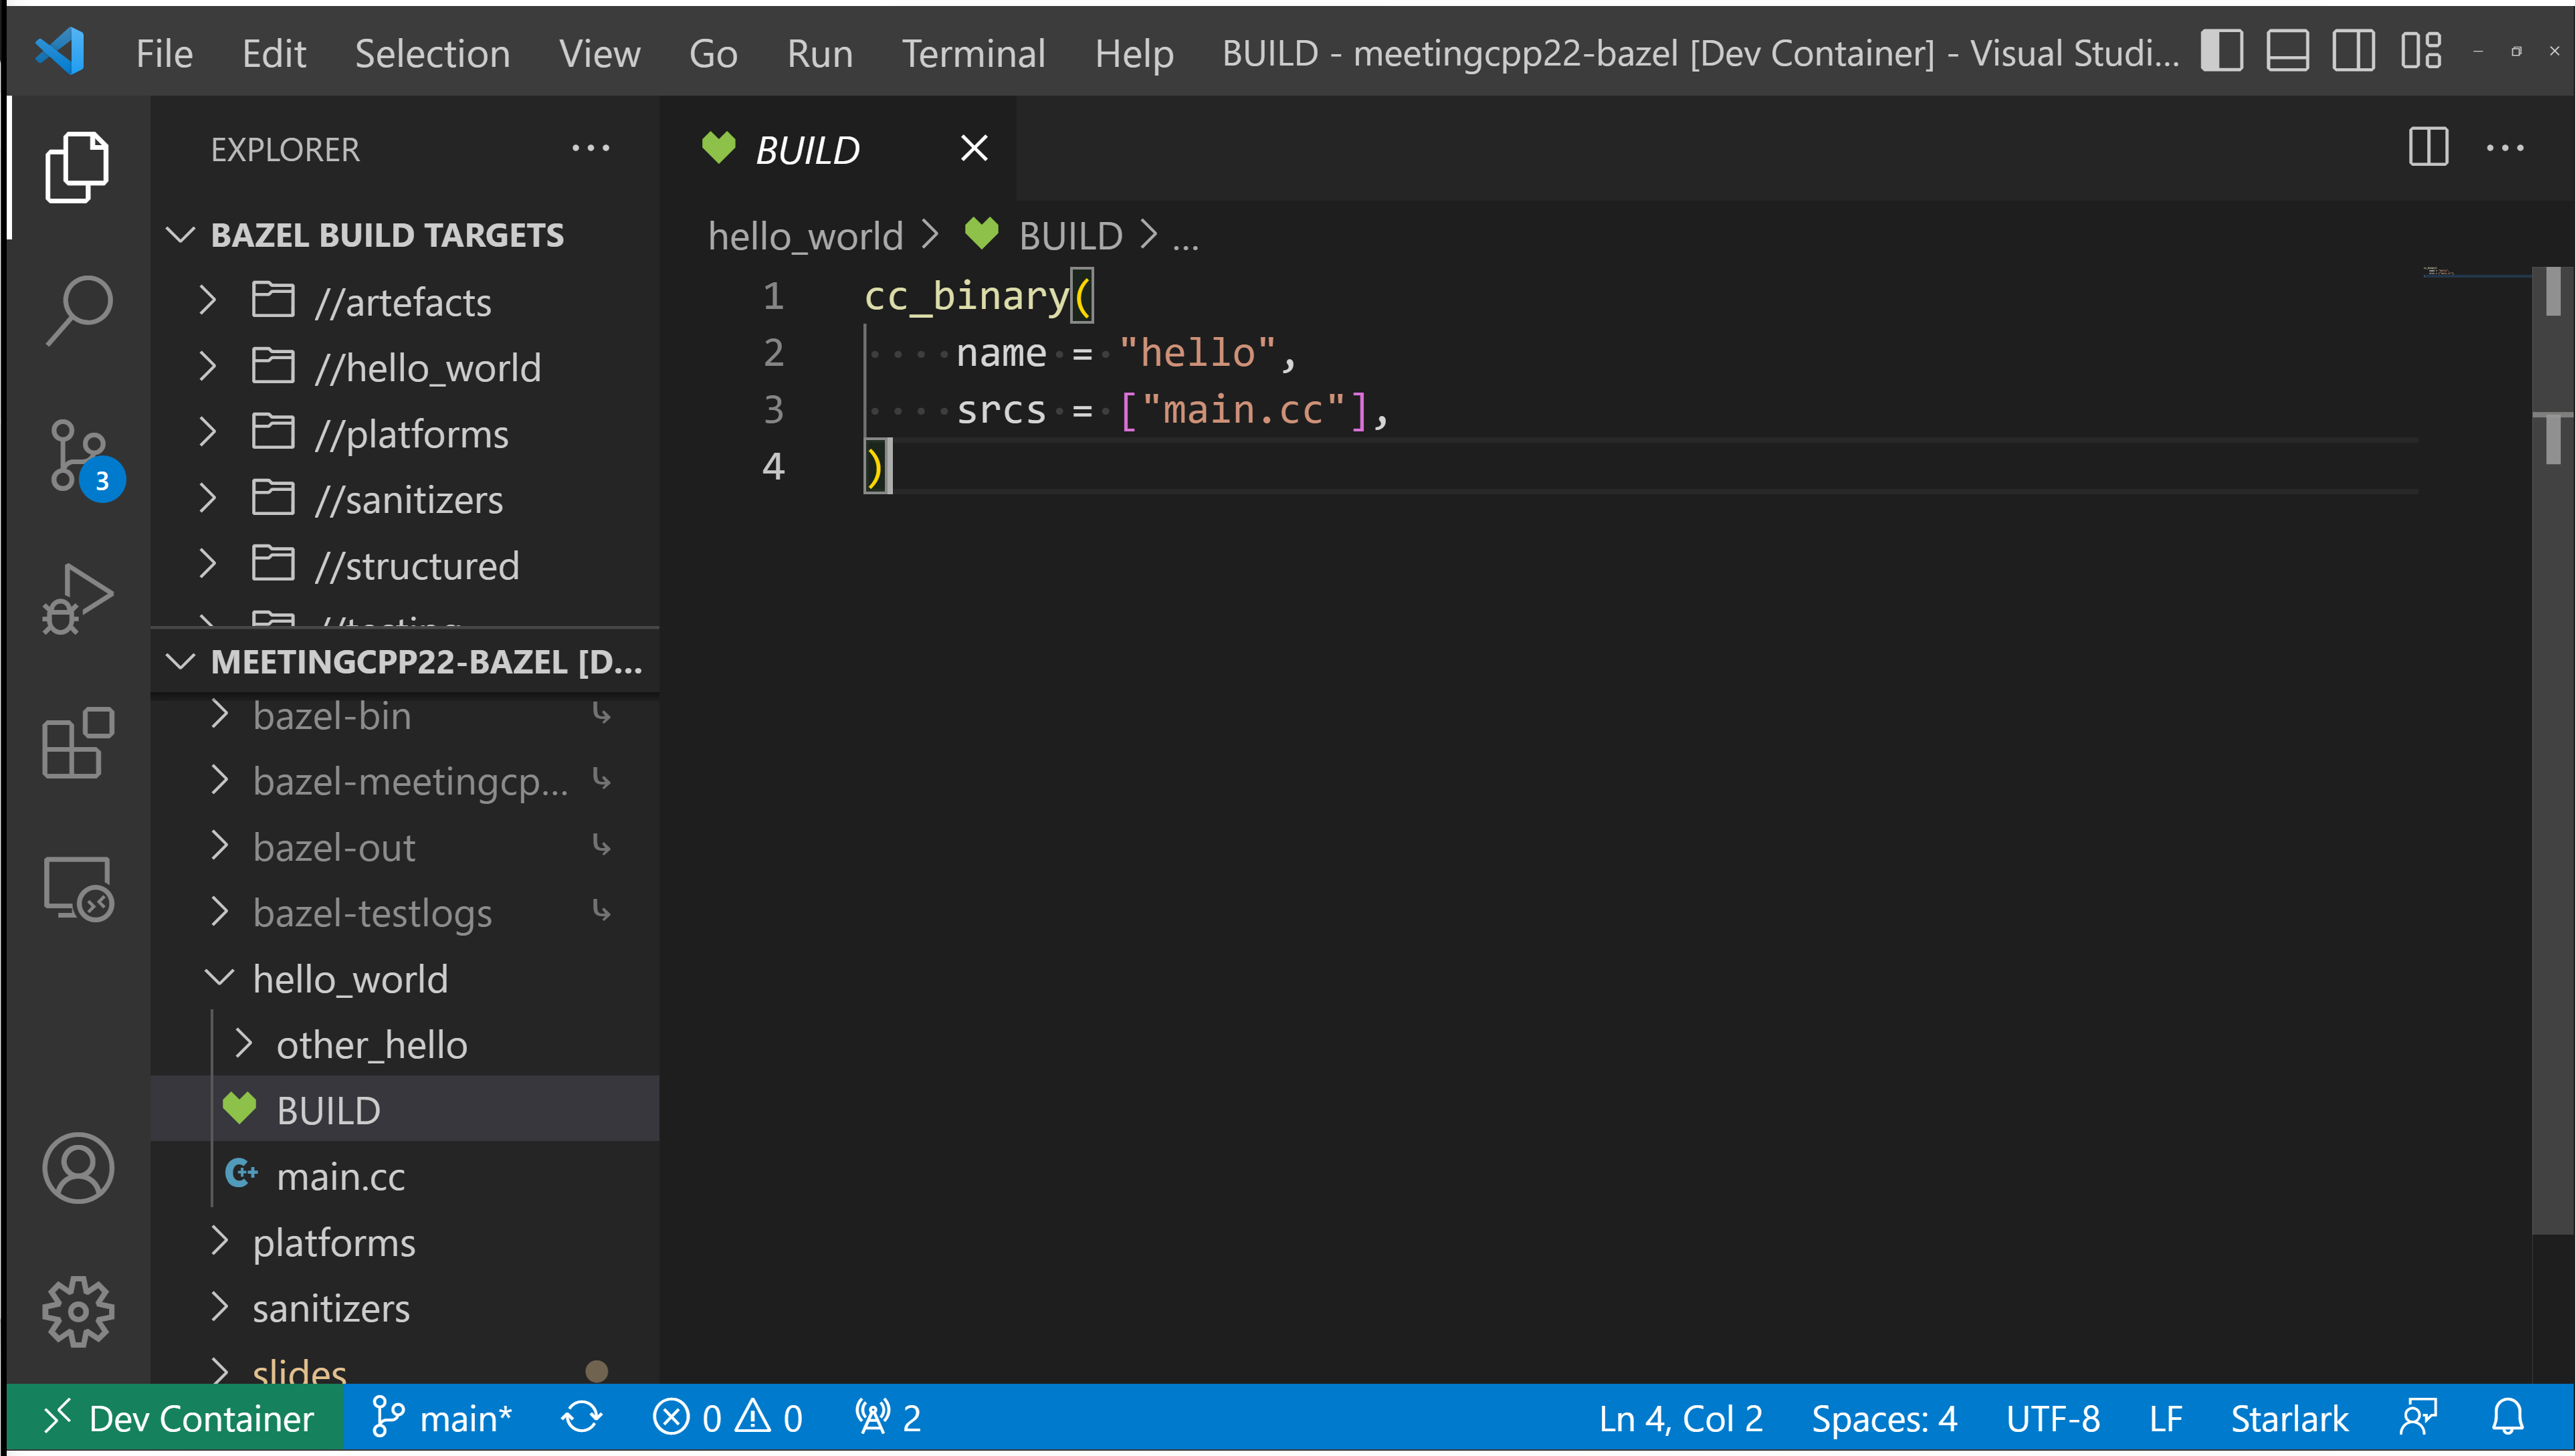
\includegraphics[width=\paperwidth]{slides/static_demos/00_06_BUILD.png}}
\begin{frame}[plain]
\end{frame}
}

{
\usebackgroundtemplate{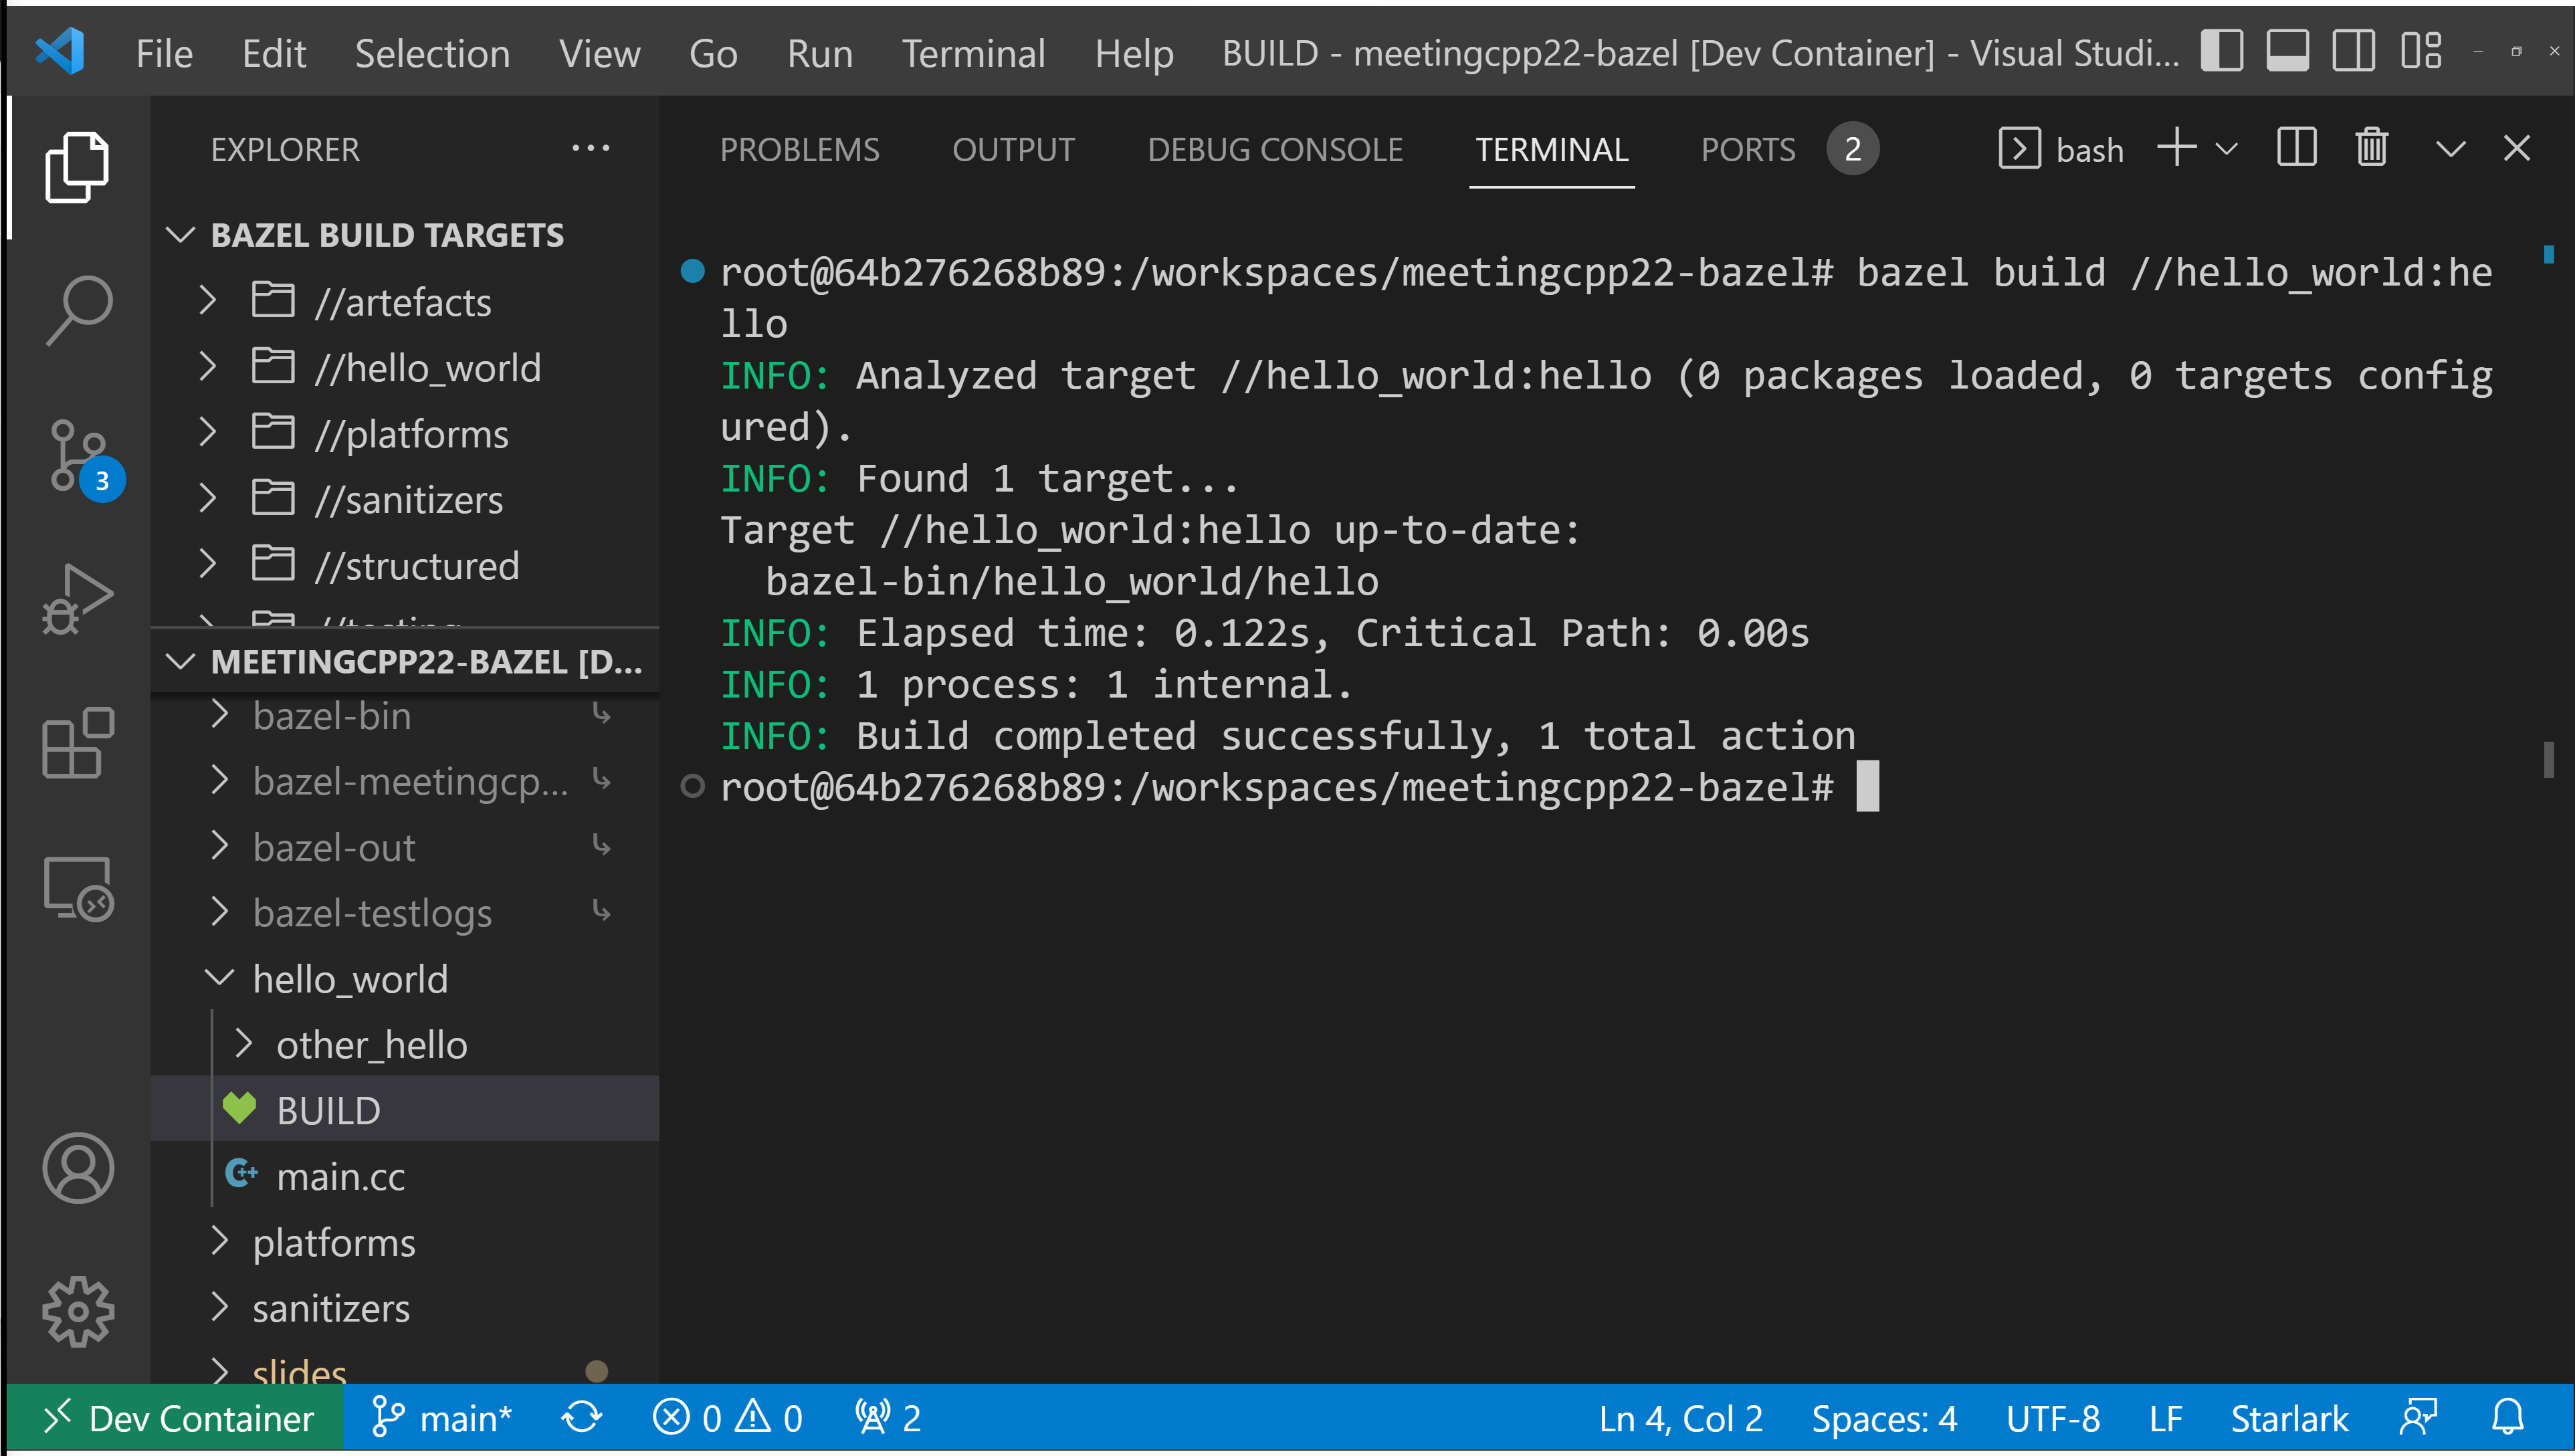
\includegraphics[width=\paperwidth]{slides/static_demos/00_07_build.png}}
\begin{frame}[plain]
\end{frame}
}

{
\usebackgroundtemplate{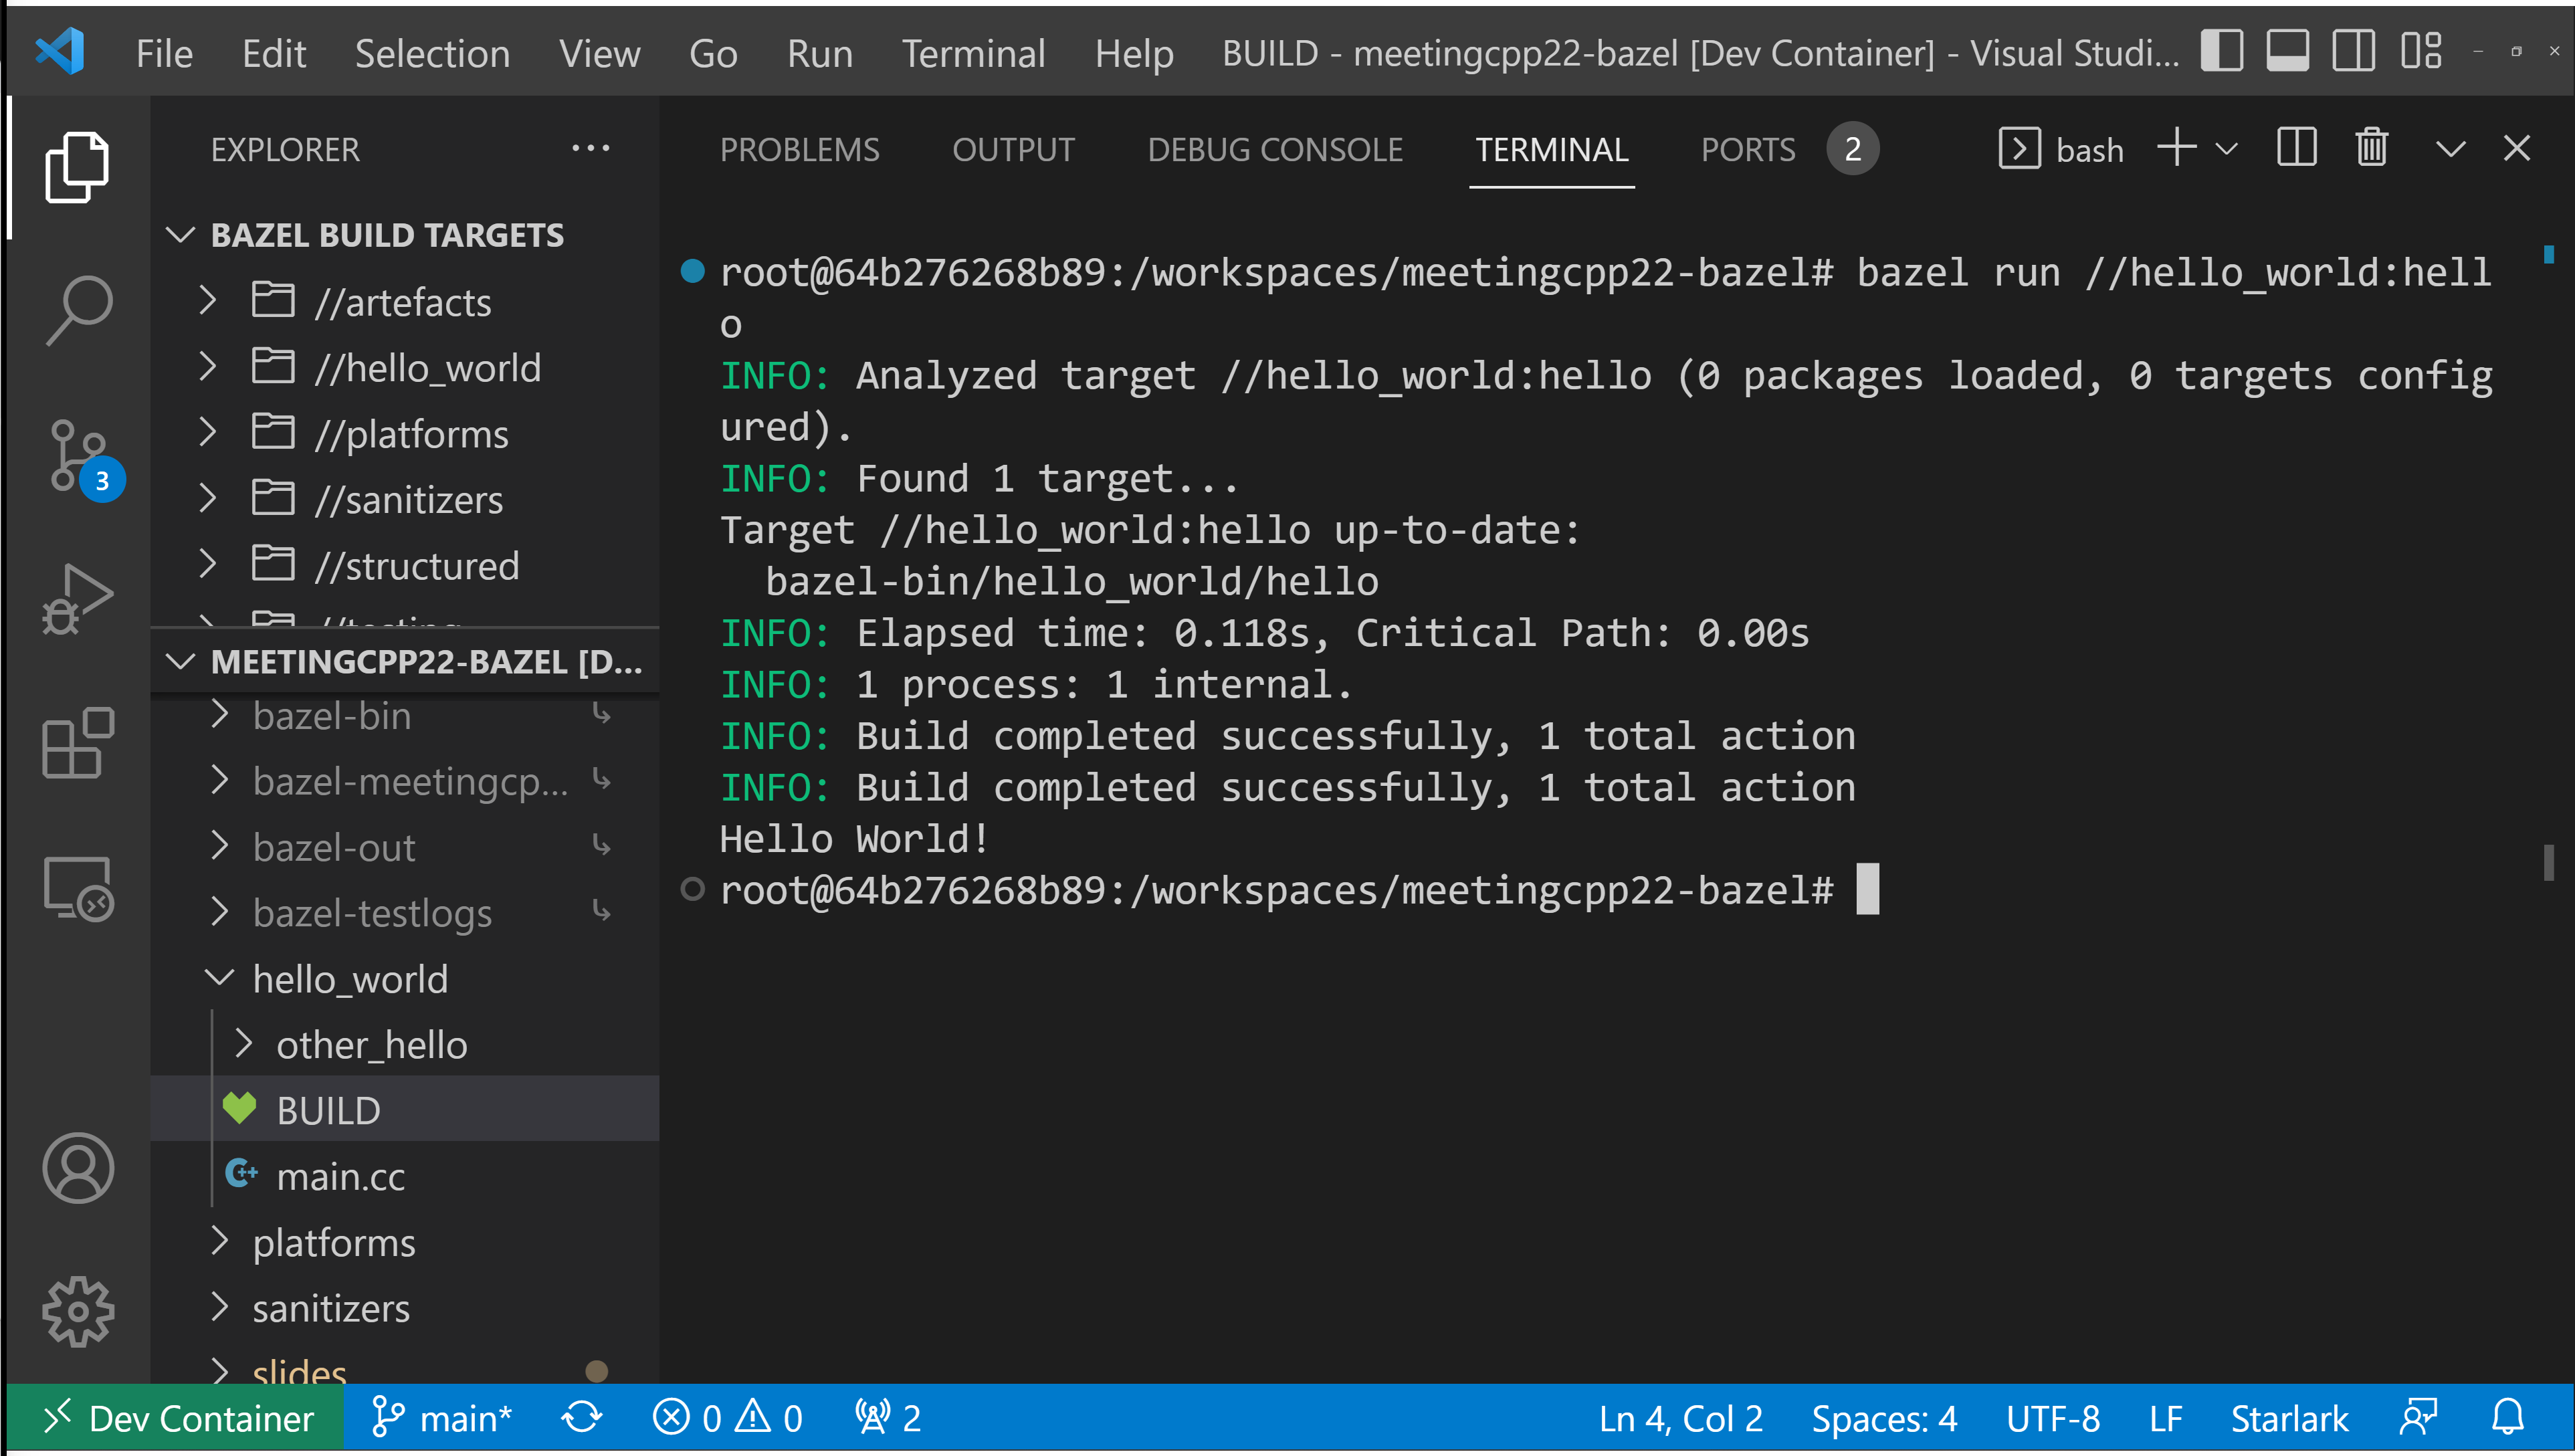
\includegraphics[width=\paperwidth]{slides/static_demos/00_08_run.png}}
\begin{frame}[plain]
\end{frame}
}

\begin{frame}{Repo, Package, Target}
\begin{center}
\begin{overprint}
\onslide<1> \huge{\texttt{@repo//package/path:target}}
\onslide<2> \huge{\texttt{@//package/path:target}}
\onslide<3>\huge{\texttt{//package/path:target}}
\onslide<4>\huge{\texttt{:target}}
\onslide<5>\huge{\texttt{//package/path:path}}
\onslide<6>\huge{\texttt{//package/path}}
\end{overprint}
\end{center}
\end{frame}

{
\usebackgroundtemplate{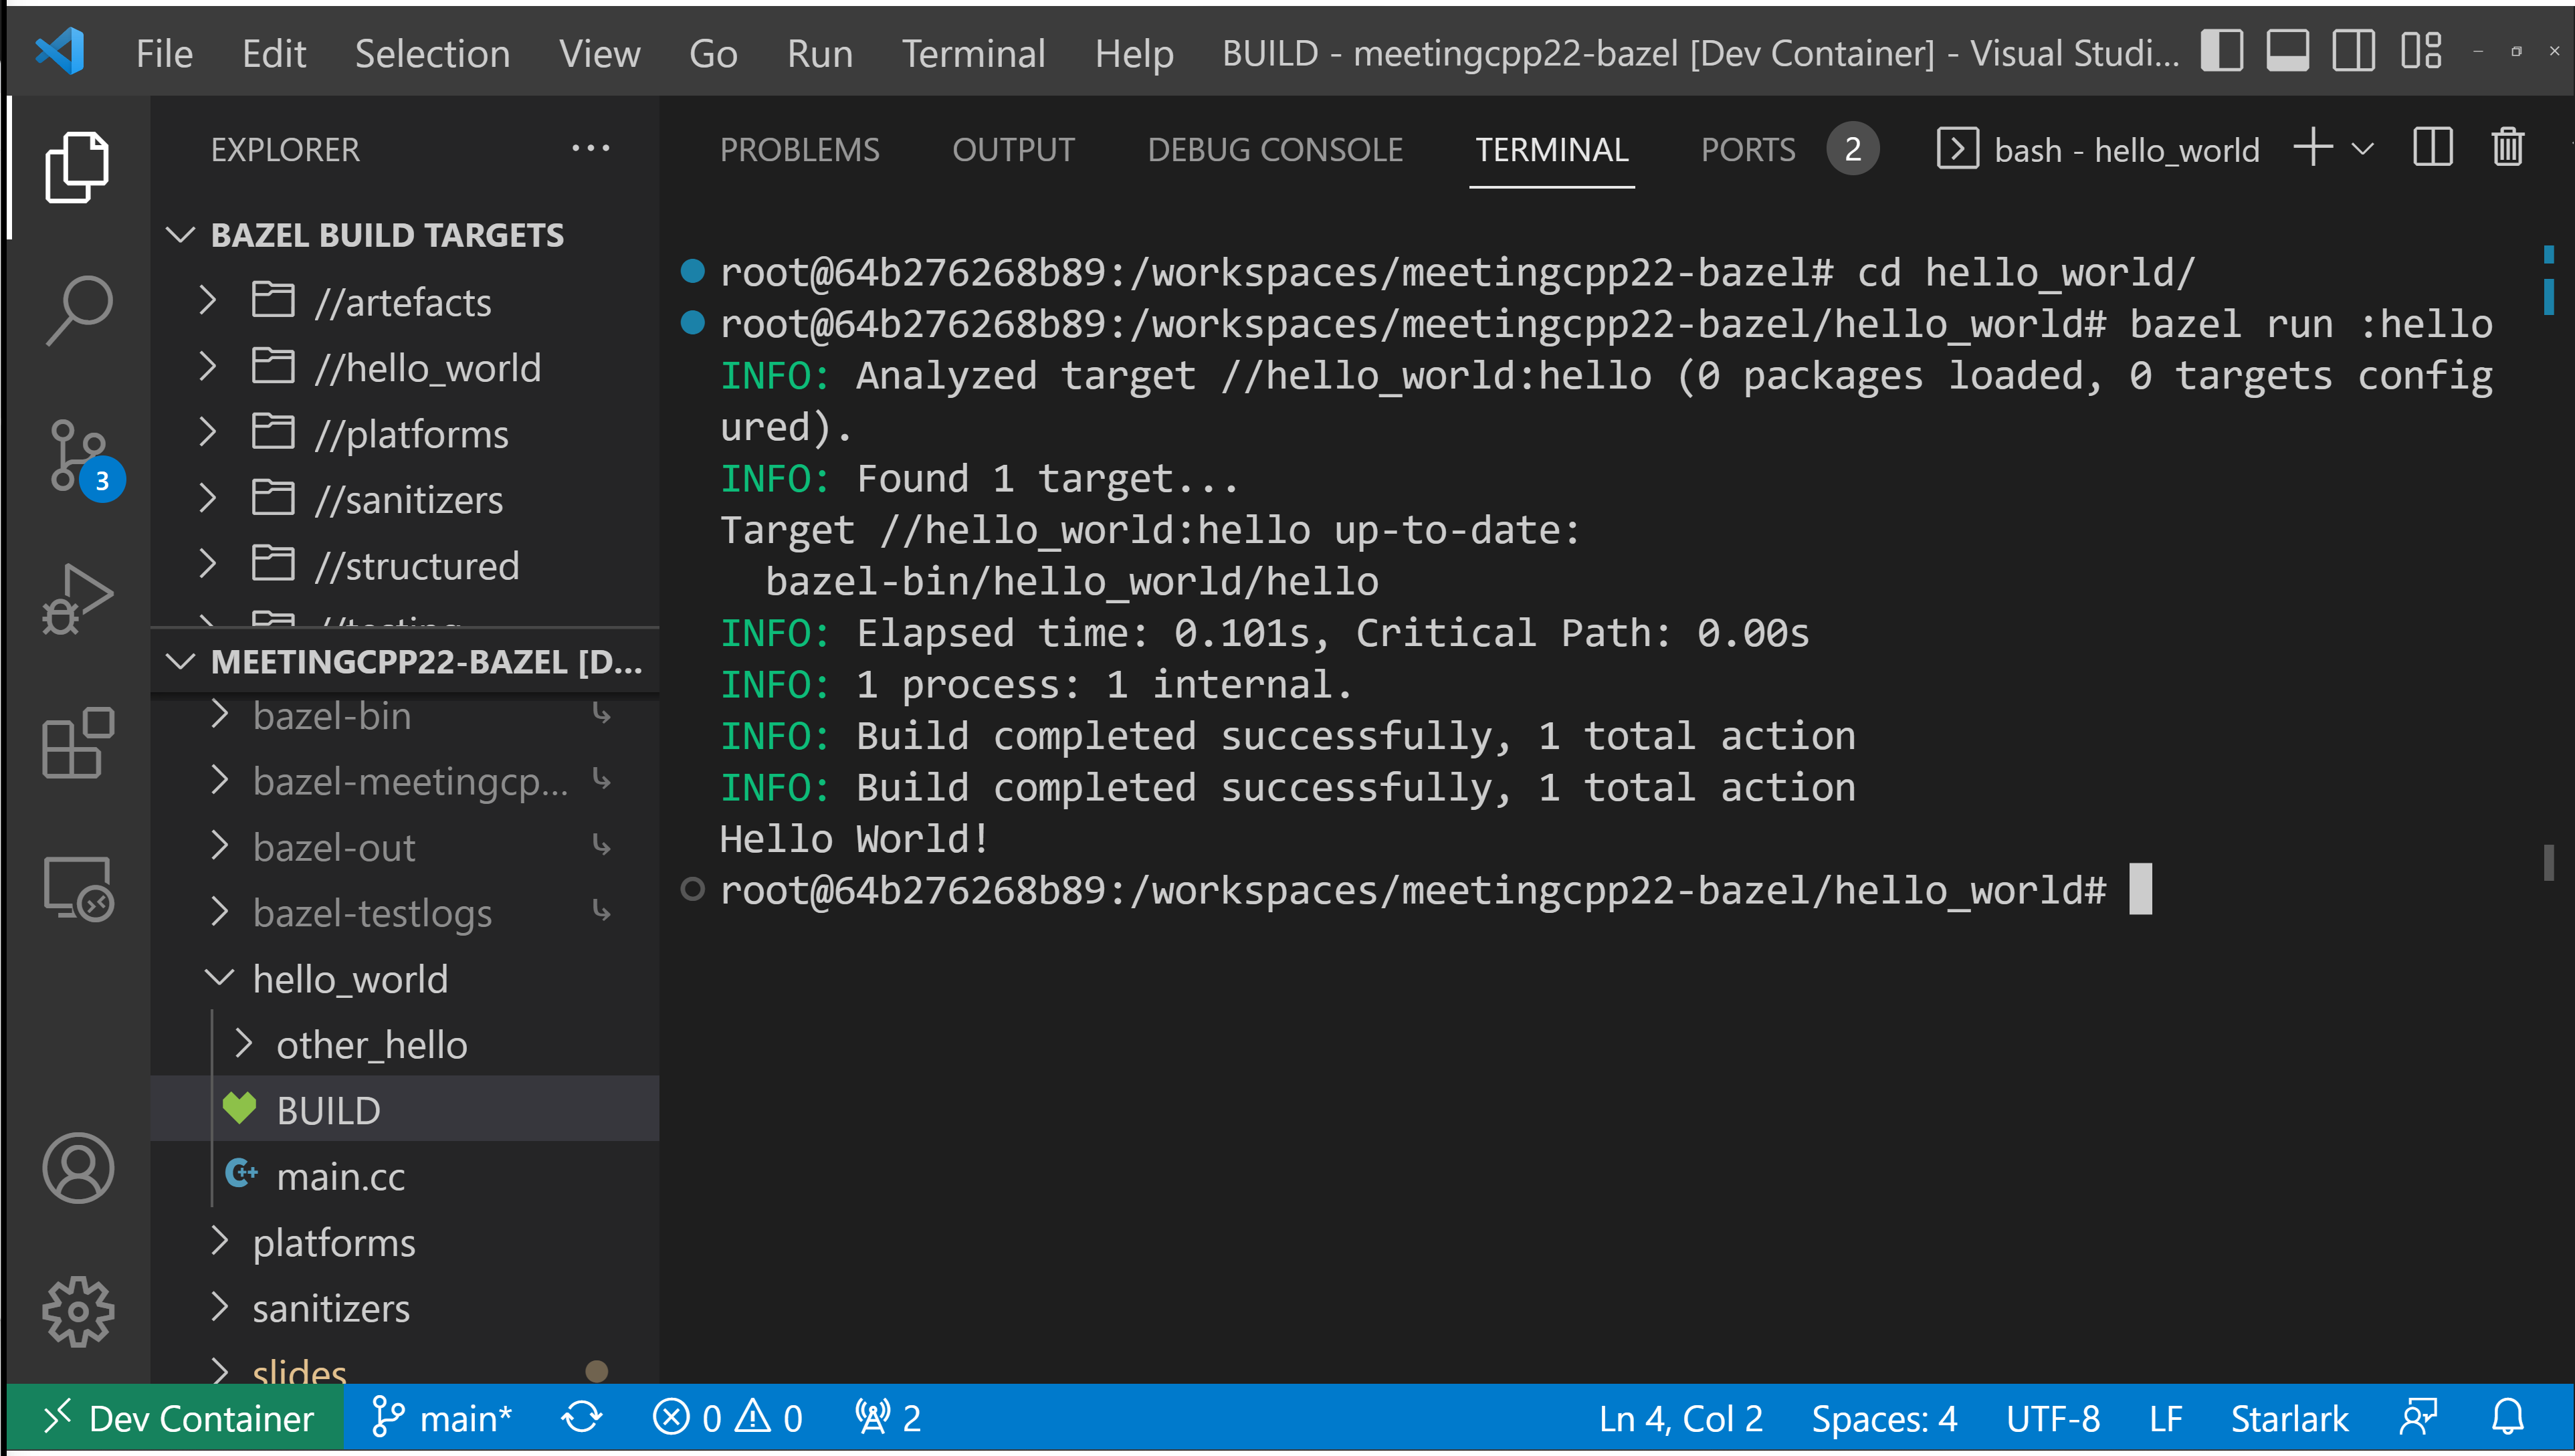
\includegraphics[width=\paperwidth]{slides/static_demos/00_09_local.png}}
\begin{frame}[plain]
\end{frame}
}

{
\usebackgroundtemplate{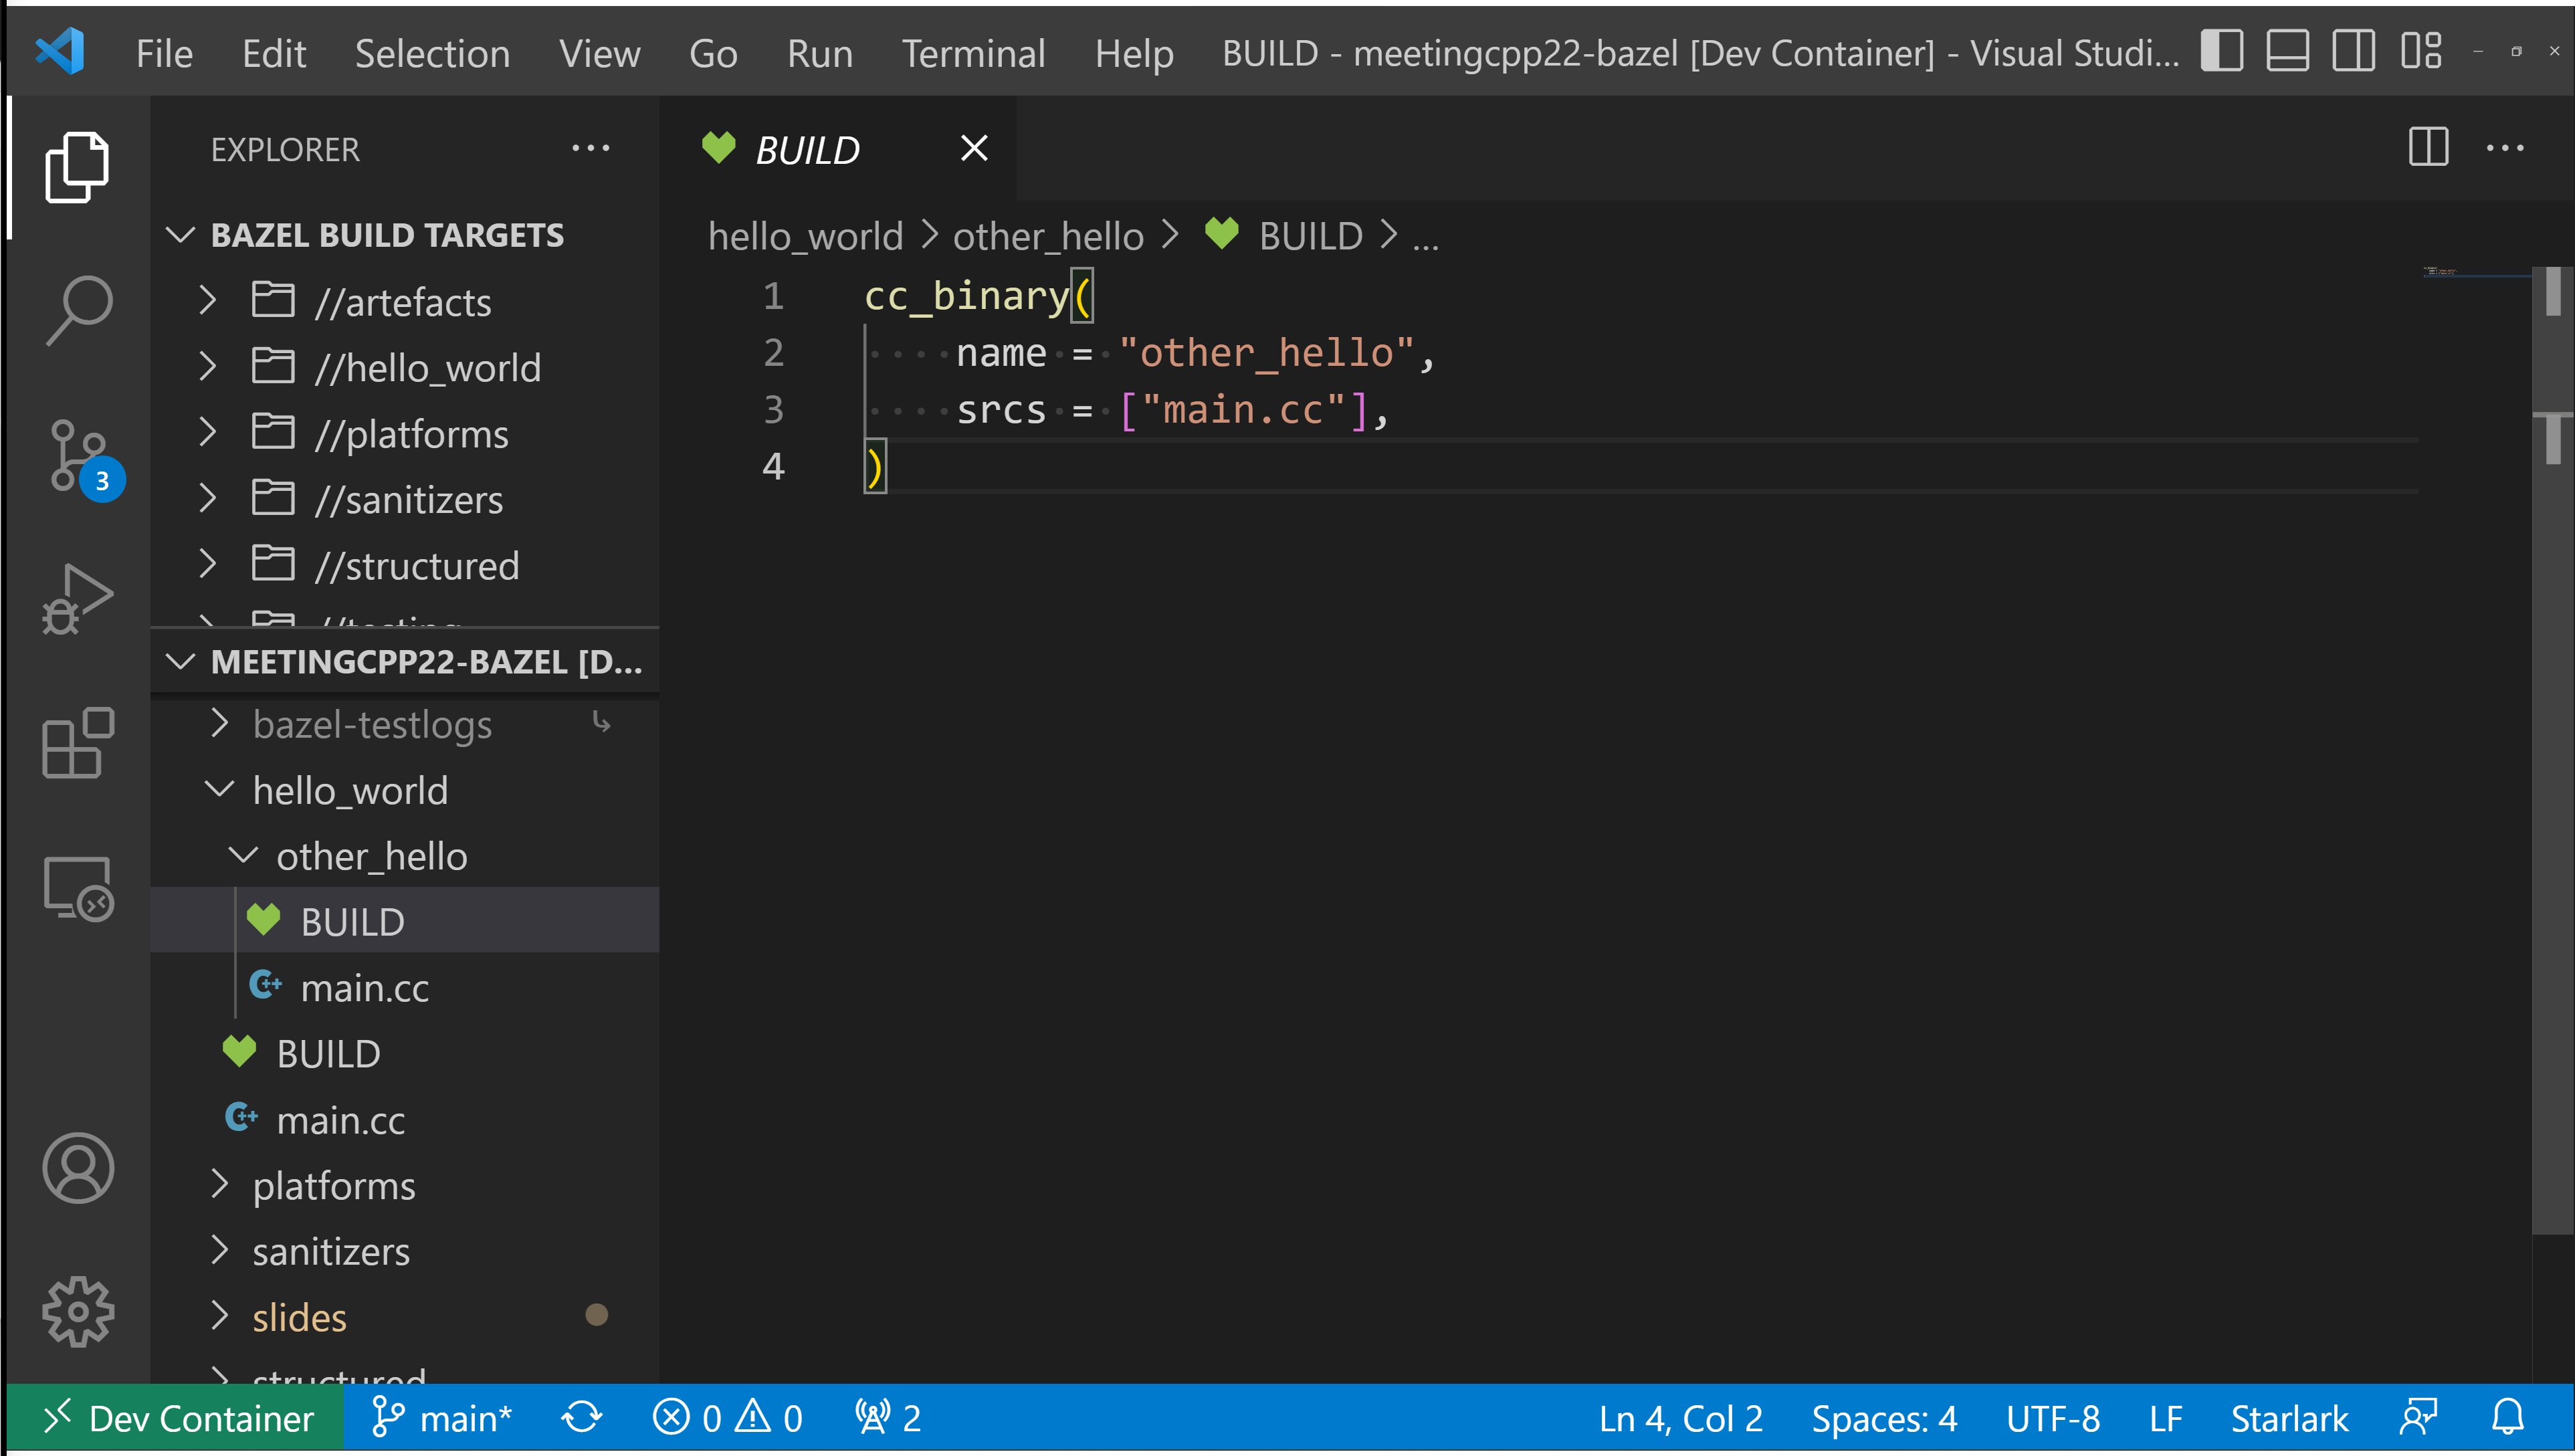
\includegraphics[width=\paperwidth]{slides/static_demos/00_10_other_hello.png}}
\begin{frame}[plain]
\end{frame}
}

{
\usebackgroundtemplate{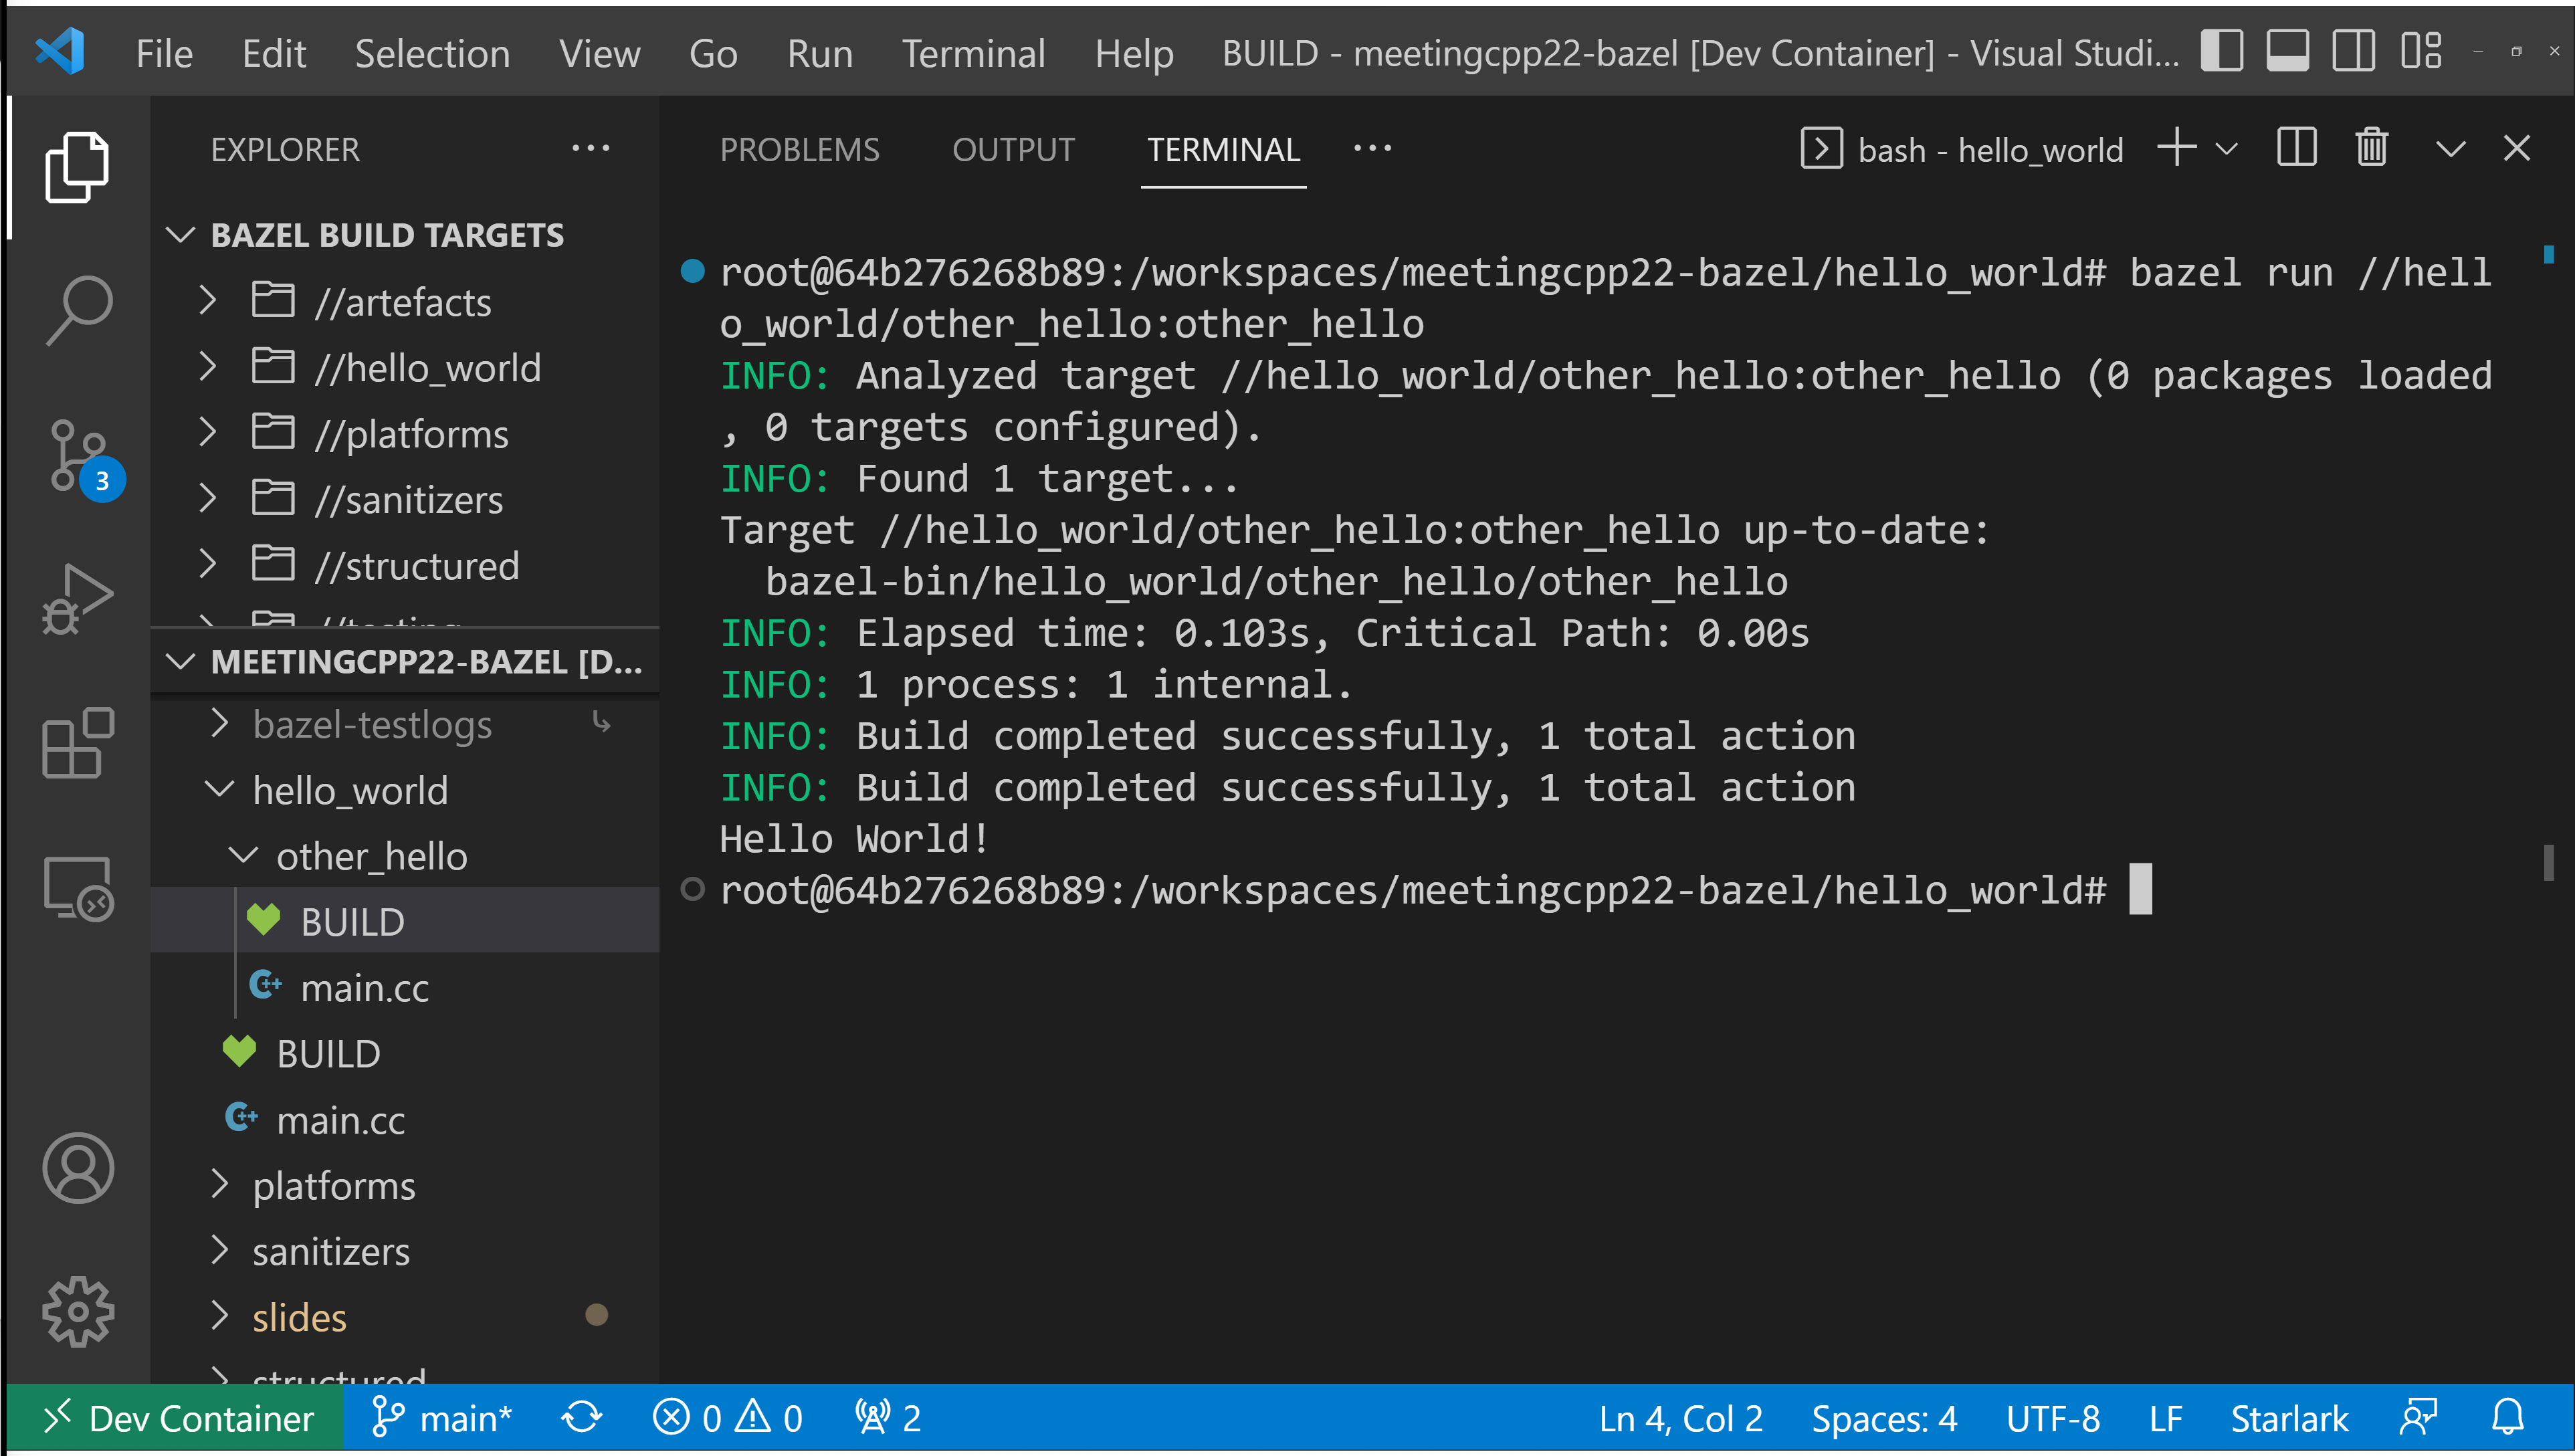
\includegraphics[width=\paperwidth]{slides/static_demos/00_11_other_run.png}}
\begin{frame}[plain]
\end{frame}
}

{
\usebackgroundtemplate{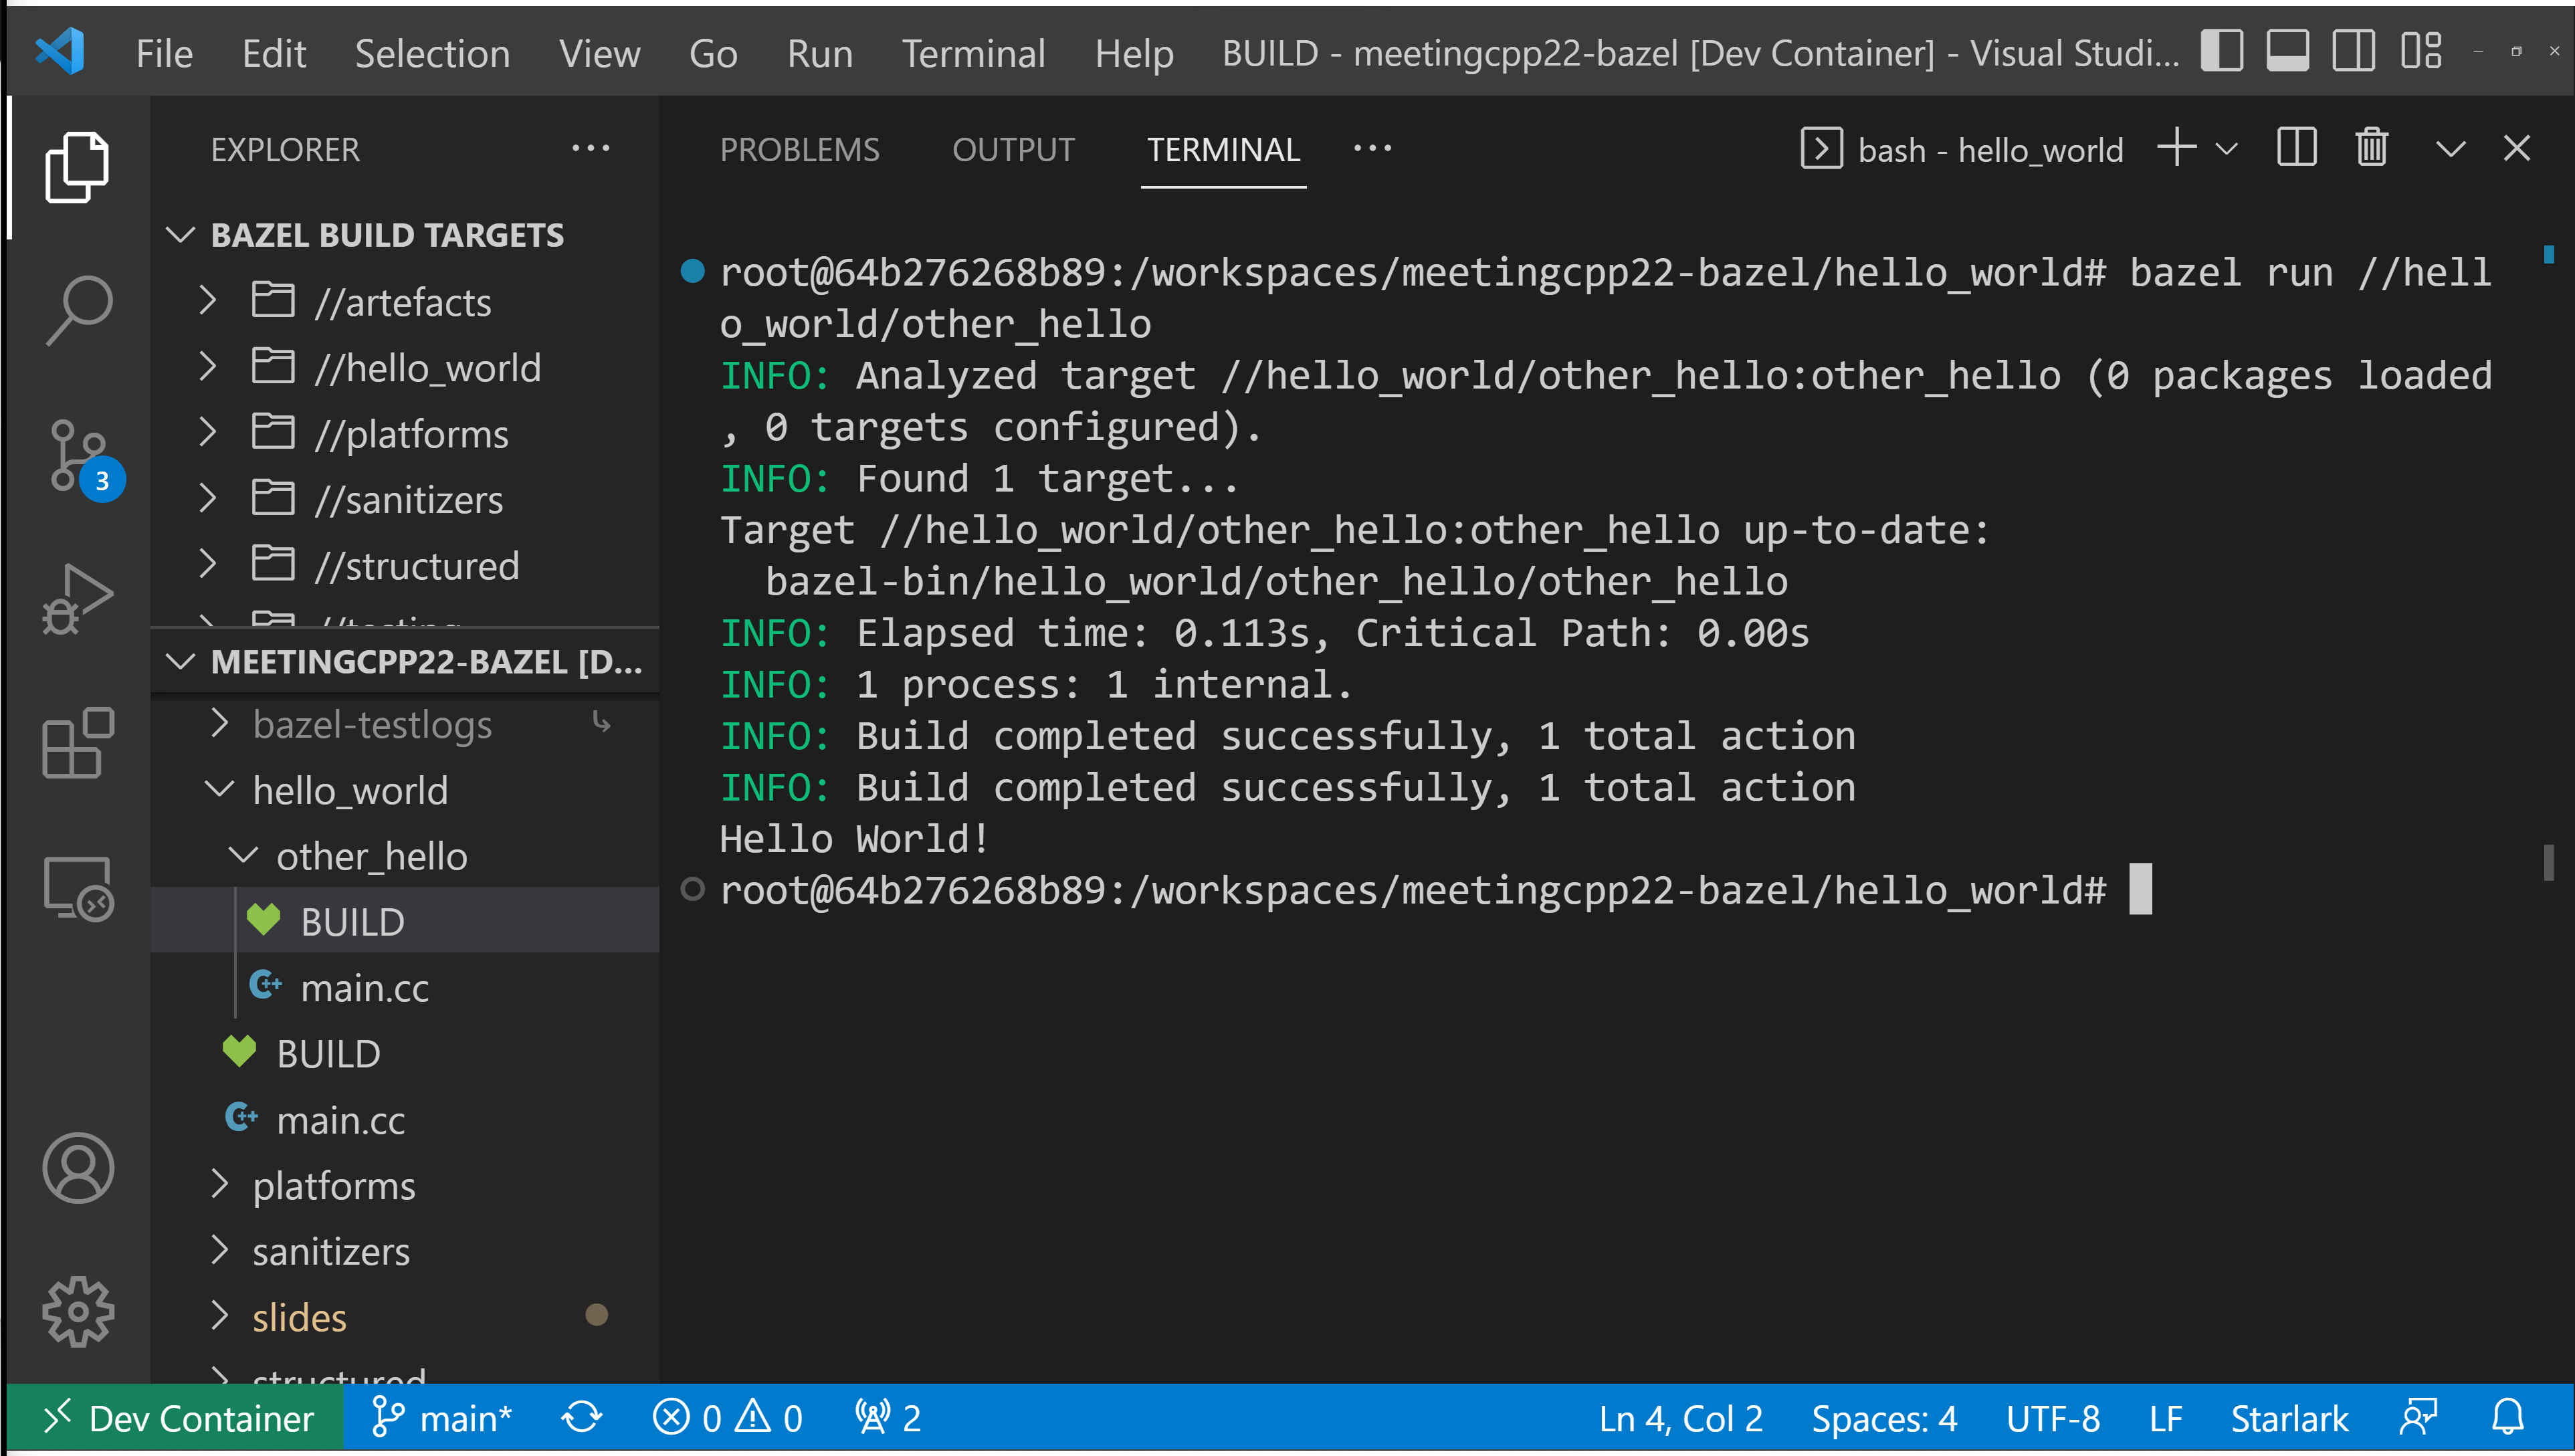
\includegraphics[width=\paperwidth]{slides/static_demos/00_12_other_run_short.png}}
\begin{frame}[plain]
\end{frame}
}



\end{document}